\documentclass[a4paper,fleqn]{cas-sc}
% Avoid 'TeX capacity exceeded [PDF object stream buffer]' on large embedded figures.
\ifdefined\pdfobjcompresslevel\pdfobjcompresslevel=0\fi
\usepackage{hyperref}
\usepackage[numbers,sort&compress]{natbib}
\usepackage{graphicx}
\graphicspath{{./}}
\usepackage{textcomp}
\usepackage{float}       % [H]: figures and tables stay at the point where they are placed
\usepackage{adjustbox}   % shrink (never enlarge) wide tables to the text width
\usepackage{url}
\hypersetup{citecolor=blue,linkcolor=blue,urlcolor=blue,breaklinks=true}

% cas-sc stores the figure position in a macro, so float.sty never sees [H] and the
% figure is deferred to the end of the document. Same environment as cas-common.sty,
% except that the position is passed explicitly and [H] closes with float.sty's \float@endH.
\makeatletter
\ExplSyntaxOn
\RenewDocumentEnvironment { figure } { O{} }
  {
    \__reset_fig:
    \bool_gset_false:N \g_fig_full_bool
    \dim_set:Nn \l_fig_width_dim { \linewidth }
    \keys_set:nn { cas / fig } { #1 }
    \csxdef{fps@figure}{\l_fig_pos_tl}
    \csgdef{figwidth}{\dim_use:N \l_fig_width_dim}
    \cs_set_eq:NN \@makecaption \__make_fig_caption:nn
    \exp_last_unbraced:Nx \@float { {figure} [ \l_fig_pos_tl ] }
     \l_fig_align_tl
     \sffamily\small
  }
  {
    \tl_if_eq:NnTF \l_fig_pos_tl { H } { \float@endH } { \end@float }
  }
\ExplSyntaxOff
\makeatother

% Headline numbers: final MM-Net (fine-tuned, cross-fitted, aligned EEG/EOG encoder; eight
% cardiorespiratory channels; cross-attention fusion), three seeds x ten patient-independent folds.
\newcommand{\mmAcc}{0.763}
\newcommand{\mmAccS}{0.756}
\newcommand{\mmMf}{0.664}
\newcommand{\mmK}{0.656}
\newcommand{\mmAuc}{0.825}
\newcommand{\mmAp}{0.487}
\newcommand{\mmRho}{0.765}
% Frozen-encoder configuration of the same architecture, used for the controlled analyses.
\newcommand{\fzAcc}{0.739}
\newcommand{\fzMf}{0.670}
\newcommand{\fzK}{0.634}
\newcommand{\fzAuc}{0.782}
\newcommand{\fzAp}{0.419}
\newcommand{\pend}[1]{\textcolor{red}{#1}}   % values still being finalised

\newcommand{\noflowAuc}{0.778}

\begin{document}
\let\WriteBookmarks\relax
\def\floatpagepagefraction{1}
\def\textpagefraction{.001}

\shorttitle{MM-Net: sleep staging and sleep apnea assessment after ischemic stroke}
\shortauthors{M. W. Suva et~al.}

\title[mode = title]{MM-Net: A Multimodal Multi-Task Network for Sleep Staging and Sleep Apnea Assessment After Ischemic Stroke}

\author[1]{Md Wahiduzzaman Suva}
\ead{26-94088-2@student.aiub.edu}


\author[1]{Esm-e Moula Chowdhury Abha}
\ead{26-94089-2@student.aiub.edu}

\author[1]{Md Imtiaj Alam Sajin}
\ead{26-94090-2@student.aiub.edu}

\author[1]{Md Iftekharul Mobin}
\cormark[1]
\ead{iftekhar.mobin@aiub.edu}

\author[2]{M. Abdullah-Al-Wadud}
\ead{mwadud@ksu.edu.sa}

\author[3]{Saifur Rahman Sabuj}
\ead{s.r.sabuj@ieee.org}

\author[4]{Jia Uddin}
\cormark[1]
\ead{jia.uddin@wsu.ac.kr}

\affiliation[1]{organization={Department of Computer Science and Engineering, American International University-Bangladesh},
    city={Dhaka},
    postcode={1229},
    country={Bangladesh}}

\affiliation[2]{organization={Department of Software Engineering, College of Computer and Information Sciences, King Saud University},
    city={Riyadh},
    postcode={11543},
    country={Saudi Arabia}}

\affiliation[3]{organization={Department of Automotive Engineering, Hanyang University},
    city={Seoul},
    postcode={04763},
    country={South Korea}}

\affiliation[4]{organization={AI and Big Data Department, Woosong University},
    city={Daejeon},
    country={Republic of Korea}}

\cortext[1]{Corresponding authors: M. I. Mobin (iftekhar.mobin@aiub.edu) and J. Uddin (jia.uddin@wsu.ac.kr).}

\begin{abstract}
Automated polysomnography after ischemic stroke presents challenges arising from altered sleep-related neural activity and concurrent respiratory disturbances. Existing stroke-specific approaches have primarily addressed sleep-stage classification, leaving the joint analysis of sleep architecture and respiratory events insufficiently investigated. Furthermore, adapting pretrained EEG encoders introduces a representation inconsistency when downstream models are trained on embeddings from previously observed patients but evaluated on unseen individuals. We propose MM-Net, a multimodal multi-task framework that addresses this inconsistency through cross-fitting and ridge-based embedding alignment. Sleep-adapted EEG--EOG representations and engineered neural descriptors are integrated with learned cardiorespiratory features through cross-attention and shared temporal modeling to support simultaneous sleep staging and respiratory-event detection. On iSLEEPS, comprising 99 patients with subacute ischemic stroke, ten-fold patient-independent evaluation achieved 76.3\% sleep-staging accuracy (Cohen's $\kappa = 0.656$) and 0.825 respiratory-event AUC, outperforming the evaluated baselines under matched protocols. Controlled experiments demonstrated that embedding alignment improved staging accuracy from 75.7\% to 76.9\% over cross-fitted adaptation without alignment. The framework also achieved 86.4\% staging accuracy on healthy Sleep-EDF, the highest reported in the study's benchmark comparison, and 80.3\% staging accuracy with 0.889 respiratory AUC on ISRUC-I, exceeding its retrained staging baselines. Without retraining, the iSLEEPS-trained model retained respiratory AUCs of 0.833 on ISRUC-I and 0.841 on UCD. These findings support representation-consistent neural adaptation and joint physiological modeling across stroke, healthy-sleep, and sleep-disorder cohorts.
\end{abstract}

\begin{keywords}
Apnea--hypopnea index \sep cardiorespiratory signals \sep EEG representation learning \sep ischemic stroke \sep multi-task learning \sep multimodal learning \sep polysomnography \sep sleep apnea \sep sleep staging
\end{keywords}

\maketitle

%=====================================================================
\section{Introduction}

Sleep disturbances are common after ischemic stroke and have been associated with neurological recovery and functional outcomes~\cite{bassetti2006sleep,denis2024sleep,tellenbach2023brainstem,johnson2010frequency}. Sleep-disordered breathing is particularly prevalent in this population, making the assessment of sleep architecture and respiratory disturbance relevant to post-stroke evaluation. Polysomnography (PSG) records the physiological information required for both assessments, including electroencephalographic (EEG), electrooculographic (EOG), electromyographic (EMG), respiratory, and cardiovascular signals. Sleep-stage scoring primarily depends on neural and muscular activity, whereas respiratory-event identification relies on changes in ventilation, respiratory effort, oxygen saturation, and related physiological responses. Their concurrent analysis therefore requires a model capable of learning from heterogeneous signals whose relevance differs across prediction tasks.

Automated sleep staging has progressed from convolutional and recurrent architectures to attention-based sequence models and pretrained neural representations~\cite{supratak2017deepsleepnet,phan2019seqsleepnet,eldele2021attnsleep,supratak2020tinysleepnet,labram2024,cbramod2025,eegpt2024,biot2023}. Multimodal approaches have expanded this direction by integrating physiological signals, temporal context, and complementary representations. Recent studies published in Biomedical Signal Processing and Control, including MMS-SleepNet~\cite{mmssleepnet2025} and CrossFusionSleepNet~\cite{crossfusionsleepnet2026}, demonstrate the growing use of physiological knowledge, modality-specific encoding, and attention-based fusion for sleep staging. Respiratory-event detection has developed alongside these methods, and joint approaches have established the feasibility of predicting sleep stages and respiratory events within a shared framework. Huttunen \emph{et al.}~\cite{huttunen2023simultaneous} evaluated simultaneous scoring in 877 clinical PSG recordings, while subsequent multi-task models have investigated related problems in other sleep populations~\cite{multitask2025elderly}. These developments establish a methodological foundation for joint sleep analysis, although their evaluation has primarily involved general sleep-disorder, suspected-apnea, or elderly cohorts.

The application of these methods to ischemic stroke introduces additional physiological and computational considerations. Cerebrovascular injury can alter sleep spindles, slow-wave activity, and hemispheric EEG characteristics~\cite{gottselig2002stroke,fernandez2019spindles,facchin2020slowwaves,simpson2023laterality,zheng2025spindles,anastasi2017bsi}, potentially affecting representations learned from healthy or conventional sleep-disorder populations. The recently released iSLEEPS dataset~\cite{maiti2026isleeps} provides multimodal overnight PSG recordings from 100 patients with ischemic stroke, including expert annotations of sleep stages and respiratory events. Its initial analysis established sleep-staging baselines for this population. Bose \emph{et al.}~\cite{bose2026gap} subsequently investigated the generalization of EEG-based staging models between healthy and stroke cohorts, reporting performance degradation and changes in the physiological patterns emphasized by the model. More recently, Alhazmi~\cite{alhazmi2026sleepstagenet} introduced SleepStageNet, a compact five-channel staging architecture evaluated on 95 iSLEEPS recordings, together with physiological attribution analyses and transfer to an independent healthy-sleep cohort. Collectively, these studies have advanced stroke-specific sleep classification and demonstrated the importance of population-dependent evaluation. The joint prediction of sleep architecture and respiratory-event onset from stroke PSG, however, remains insufficiently investigated.

This gap also raises a question concerning the organization of multimodal physiological information. Neural and cardiorespiratory signals provide different evidence for sleep state and respiratory disturbance, although both tasks depend on temporal context and interactions among physiological systems. A shared model must therefore integrate information across modalities while retaining features relevant to individual outputs. Furthermore, respiratory-event annotations are closely associated with recorded airflow and respiratory-effort signals. Improved discrimination from multimodal inputs cannot, by itself, establish whether a model has learned complementary physiological relationships or relies predominantly on channels directly associated with event scoring. Controlled modality and channel interventions are necessary to distinguish these contributions and characterize the dependence of each task on its available signals.

A separate methodological difficulty arises when pretrained EEG encoders are adapted to a clinical cohort and subsequently used to train a downstream prediction model. Adaptation can improve the relevance of learned representations to post-stroke sleep, but embeddings generated for patients used during encoder training may differ from those produced for previously unseen patients. Cross-fitting addresses the in-sample dependence by generating downstream training embeddings from encoders that have not observed the corresponding patients, consistent with established principles of stacked generalization~\cite{chernozhukov2018dml}. However, independently adapted encoders may produce representations in different feature spaces, introducing an additional inconsistency with the encoder used at deployment. Consequently, reliable integration requires both out-of-sample representation generation and alignment with the deployed encoder's embedding space. The contribution of these operations can be evaluated directly through controlled encoder-integration comparisons.

To address these problems, we develop MM-Net, a multimodal multi-task framework for joint sleep-stage classification and respiratory-event-onset detection. The neural stream combines physiologically defined descriptors with embeddings from a sleep-adapted LaBraM encoder~\cite{labram2024}. Cross-fitting produces out-of-sample representations for downstream training, and ridge-based alignment maps these representations into the embedding space of the encoder used for inference. A complementary convolutional stream extracts information directly from cardiorespiratory waveforms. Cross-attention and bidirectional temporal modeling integrate the representations, while task-specific prediction pathways support five-class sleep staging and respiratory-event scoring. A direct cardiorespiratory pathway preserves respiratory information for event detection, and the resulting scores additionally support patient-level apnea--hypopnea index estimation.

We evaluate the framework using patient-independent protocols across stroke, healthy-sleep, and sleep-disorder populations. The primary analysis uses 99 unique iSLEEPS recordings after a duplicate-record audit, supported by matched staging and respiratory baselines, controlled encoder comparisons, and physiological signal interventions. Controlled experiments further establish the contribution of embedding alignment to sleep-adapted encoder integration. To examine applicability beyond the development population, the framework is separately evaluated on Sleep-EDF and ISRUC-Sleep. Additional experiments assess transfer of the iSLEEPS-trained model to independent cohorts without retraining. Together, these evaluations investigate both the methodological contribution of representation-consistent adaptation and the applicability of joint physiological modeling across different sleep populations.

The principal contributions of this study are threefold:

\begin{enumerate}

\item Representation-consistent integration of sleep-adapted EEG features. We address the mismatch arising when an EEG encoder adapted on training patients supplies representations to a downstream model evaluated on unseen patients. A cross-fitting and embedding-alignment procedure integrates out-of-sample neural representations into a common deployment space, enabling the downstream framework to benefit from sleep-specific adaptation without relying on in-sample encoder outputs during training.

\item Task-specialized multimodal modeling of post-stroke sleep physiology. We develop a unified framework for sleep-stage classification and respiratory-event detection that combines neural and cardiorespiratory representations through shared temporal modeling while retaining task-specific respiratory information. This design enables concurrent characterization of sleep architecture and respiratory disturbances in subacute ischemic stroke, with patient-level AHI estimation as an additional output.

\item Evidence for physiological specialization and cross-cohort applicability. Through controlled signal interventions and patient-independent evaluations, we examine the dependence of each prediction task on its physiological inputs and establish the performance of the integrated framework against matched baselines. Independent-cohort experiments further assess the transfer of the learned representations beyond the stroke population.

\end{enumerate}

The remainder of this paper presents the related literature, datasets, proposed methodology, experimental evaluation, and discussion of the findings.

%=====================================================================
\section{Related Work}
\label{sec:related}

\subsection{Automatic Sleep Staging}

Automatic sleep staging has progressed from feature-based classifiers to deep
models that learn temporal and spectral representations directly from PSG
signals. DeepSleepNet combines convolutional feature extraction with recurrent sequence modeling~\cite{supratak2017deepsleepnet}, and SeqSleepNet formulates sleep staging as sequence-to-sequence classification across consecutive epochs~\cite{phan2019seqsleepnet}. AttnSleep uses multi-resolution convolution and
attention to capture complementary temporal characteristics
~\cite{eldele2021attnsleep}, and TinySleepNet reduces model complexity while
retaining recurrent modeling of stage transitions
~\cite{supratak2020tinysleepnet}. U-Time approaches staging as dense
time-series segmentation~\cite{perslev2019utime}, whereas XSleepNet combines
raw-signal and spectral representations within a common sequence model
~\cite{phan2021xsleepnet}.

More recent work has expanded the range of temporal models and learned
representations. SleepTransformer applies attention-based sequence modeling
~\cite{sleeptransformer2022}, L-SeqSleepNet extends modeling across longer
sleep-stage sequences~\cite{lseqsleepnet2023}, and ZleepAnlystNet and
FlexSleepTransformer investigate alternative training strategies and flexible
channel configurations
~\cite{jirakittayakorn2024zleep,guo2024flexsleep}. State-space architectures
based on Mamba have also been explored for sleep staging
~\cite{gu2023mamba,bitmamsleep2024}. In parallel, large pretrained EEG models
such as LaBraM, CBraMod, EEGPT, and BIOT provide representations learned from
substantially larger collections of neural recordings
~\cite{labram2024,cbramod2025,eegpt2024,biot2023}. Such encoders are typically
used frozen or fine-tuned end to end for a single task. Using a fine-tuned
encoder as the input of a second model trained on the same patients raises the
requirement addressed by stacked generalization and cross-fitting, namely that the
second model be trained on out-of-sample first-stage outputs
~\cite{chernozhukov2018dml}.

Most of these developments have been established on healthy or general sleep
datasets. Performance can change substantially when models are transferred
across cohorts because acquisition protocols, channel configurations, patient
characteristics, and sleep physiology differ between datasets
~\cite{guillot2023transfer}. This issue is especially relevant after stroke,
where the neural patterns used in conventional sleep staging may themselves be
altered by neurological injury.

\subsection{Multimodal and Joint PSG Analysis}

Clinical PSG contains several complementary physiological modalities, and a
parallel line of work has examined how these signals can be incorporated into
automatic sleep analysis. U-Sleep, for example, was developed to operate across
different EEG and EOG derivations and multiple sleep cohorts
~\cite{perslev2021usleep}. Other multimodal approaches combine neural, ocular,
muscular, cardiac, or respiratory signals through early fusion,
modality-specific encoders, or higher-level feature fusion. Recent work has also extended representation learning across PSG modalities, including SleepFM~\cite{sleepfm2026}. Cross-scale representations, self-supervised learning, and standardized sleep benchmarks have further broadened the range of models evaluated across datasets~\cite{csbrain2025,sleepyland2026,estevan2025ssl}.

Joint modeling of sleep stage and sleep-related disorders has received less
attention than sleep staging alone. Huttunen \emph{et al.}
~\cite{huttunen2023simultaneous} trained a single network for simultaneous
sleep-stage and respiratory-event scoring across 877 clinical recordings and
examined input configurations ranging from pulse oximetry to a broader PSG
montage. Multi-task approaches combining sleep staging with apnea-related
prediction have subsequently been investigated in other clinical populations
~\cite{multitask2025elderly}. These studies demonstrate that the two outputs can
be learned within a common model, but they have primarily been evaluated in
suspected-apnea, elderly, or general sleep populations.

An additional question in multimodal modeling is whether improved predictive
performance reflects complementary information across modalities or strong
dependence on a particular signal. This distinction is important when different
outputs are associated with different physiological systems. EEG, EOG, and EMG
contain information directly related to sleep state, whereas airflow,
respiratory effort, oxygen saturation, and cardiac activity characterize
different aspects of respiratory disturbance. Aggregate multimodal performance
alone does not establish how these signal groups contribute to individual
outputs.

\subsection{Respiratory-Event Detection}

Automated analysis of sleep-disordered breathing has largely developed as a
separate task. Apnea and hypopnea detectors commonly use airflow, thoracic and
abdominal respiratory effort, oxygen saturation, and ECG-derived cardiac
measures. These signals describe different stages of the physiological response:
airflow reflects reduction or cessation of ventilation, respiratory effort
provides information about continued or absent breathing effort, and oximetry
captures the subsequent change in blood oxygenation. Oxygen desaturation also
forms part of the clinical criteria used in hypopnea scoring
~\cite{aasm2023manual}. End-to-end deep models have also been developed for
respiratory-event scoring, including detection from a single respiratory-effort
belt~\cite{nassi2022effortbelt}. Biswal \emph{et al.}~\cite{biswal2018expert}
trained a recurrent--convolutional network to jointly score sleep stages, apnea
events, and limb movements from clinical PSG.

Respiratory-event models are typically optimized independently of sleep
staging and often operate on temporal resolutions different from the 30-s epoch
used for stage classification. Joint models reduce this separation by learning
both outputs from the same recording, but the interpretation of the respiratory
output requires particular care when the model has access to signals involved
in event annotation. Evaluating the contribution of individual respiratory
signals therefore provides information that overall discrimination metrics
alone cannot supply.

\subsection{Sleep and Sleep-Disordered Breathing After Stroke}

Sleep physiology is frequently altered after stroke, and sleep disturbances
have been associated with neurological and functional recovery
~\cite{bassetti2006sleep,denis2024sleep,tellenbach2023brainstem}. Changes in
sleep-related neural activity have also been reported after cerebrovascular
injury. Previous studies describe alterations in sleep spindles, slow-wave activity, and related electrophysiological patterns~\cite{gottselig2002stroke,fernandez2019spindles,simpson2023laterality,facchin2020slowwaves,zheng2025spindles}; quantitative EEG measures such as the brain symmetry index have also been examined in relation to hemispheric injury~\cite{anastasi2017bsi}. These changes make
stroke sleep a distinct setting for models whose representations were
developed predominantly on non-stroke populations.

Sleep-disordered breathing is also common during the subacute phase, so sleep
state and respiratory disturbance coexist within the same clinical recording.
Despite this overlap, automated stroke-specific sleep analysis remains limited.
The iSLEEPS dataset introduced a dedicated PSG resource for subacute ischemic
stroke and reported baseline sleep-staging performance
~\cite{maiti2026isleeps}; subsequent work has further examined the behavior of
deep staging models on this cohort~\cite{bose2026gap}. Existing stroke-specific
studies have therefore concentrated primarily on sleep-stage classification.
Joint epoch-level modeling of sleep stage and respiratory disturbance, together
with controlled analysis of the neural and cardiorespiratory information
supporting each output, remains insufficiently characterized in this
population.

%=====================================================================
\section{Datasets and Preprocessing}
\label{sec:data}

Four publicly available polysomnography datasets are used in this study (Table~\ref{tab:datasets}):
iSLEEPS~\cite{maiti2026isleeps}, Sleep-EDF
~\cite{kemp2000sleepedf,goldberger2000physionet}, ISRUC-Sleep
~\cite{khalighi2016isruc} with its three subgroups, and the St Vincent's
University Hospital / University College Dublin sleep apnea database (UCD)
~\cite{ucddb2007}. iSLEEPS is the primary cohort used for model development and
patient-independent evaluation. Sleep-EDF is used as a healthy-sleep reference
for implementation checks, transfer experiments, and subject-independent
evaluation of the staging model outside the stroke cohort. ISRUC-Sleep provides
independent sleep-disorder and healthy cohorts with both sleep-stage and
respiratory-event annotations; it is used both to train and evaluate MM-Net
under subject-independent cross-validation and to test the iSLEEPS-trained model
without retraining. UCD provides a further sleep-apnea cohort recorded on a
different acquisition system and is used for transfer only. No external cohort is
used to select the reported iSLEEPS model configuration.

\begin{table}[H]
\caption{Datasets used in the study and their roles in the evaluation.}
\label{tab:datasets}
\centering
\small
\setlength{\tabcolsep}{4pt}
\begin{tabular}{p{0.21\columnwidth} p{0.24\columnwidth}
                p{0.18\columnwidth} p{0.27\columnwidth}}
\toprule
Dataset & Population & Data used & Role \\
\midrule
iSLEEPS~\cite{maiti2026isleeps}
& Subacute ischemic stroke
& 99 patients
& Development and in-domain evaluation \\

Sleep-EDF~\cite{kemp2000sleepedf,goldberger2000physionet}
& Healthy sleep
& 40 recordings
& Reimplementation checks, healthy-sleep reference, and external staging \\

ISRUC-Sleep I~\cite{khalighi2016isruc}
& Sleep disorders
& 100 patients
& Cross-validation and transfer (staging, respiratory, AHI) \\

ISRUC-Sleep II~\cite{khalighi2016isruc}
& Sleep disorders
& 8 subjects, two nights each
& Cross-validation and transfer \\

ISRUC-Sleep III~\cite{khalighi2016isruc}
& Healthy
& 10 subjects
& Cross-validation and transfer \\

UCD~\cite{ucddb2007}
& Suspected sleep apnea
& 25 patients
& Transfer (staging, respiratory, AHI) \\
\bottomrule
\end{tabular}
\end{table}

\subsection{iSLEEPS: Primary Stroke Cohort}

The iSLEEPS dataset contains overnight PSG from 100 patients with subacute
ischemic stroke~\cite{maiti2026isleeps}. The released cohort has a mean age of
$50.5$ years and includes 77 male and 23 female participants. Sleep is scored
into the five AASM stages: Wake (W), N1, N2, N3, and rapid-eye-movement (REM)
sleep. Respiratory events are also annotated throughout the recordings.

An audit performed before cross-validation identified the records of SN15 and
SN28 as byte-identical. Retaining both identifiers could place the same
recording in different patient-level folds. One member of the duplicate pair
was therefore removed before constructing the evaluation splits, leaving
$N=99$ patients and $92{,}560$ 30-s epochs for the analyses reported here.

The resulting sleep-stage distribution is shown in
Table~\ref{tab:dist}. N2 accounts for the largest proportion of epochs, and N1 and N3 are the least frequent stages. Respiratory-event onsets are marked in $16.0\%$ of all
epochs. At the patient level, the fraction of event-positive epochs ranges from
$0$ to $60.5\%$; 80 of the 99 patients have respiratory events in more than
$5\%$ of their epochs, and the median burden is $13\%$
(Figure~\ref{fig:prev}).

\begin{table}[H]
\caption{Sleep-stage distribution in the analyzed iSLEEPS cohort
($N=99$; $92{,}560$ epochs).}
\label{tab:dist}
\centering
\begin{tabular}{lccccc}
\toprule
Stage & W & N1 & N2 & N3 & REM \\
\midrule
Share (\%) & 26.7 & 10.1 & 42.3 & 8.9 & 12.1 \\
\bottomrule
\end{tabular}
\end{table}

\begin{figure}[pos=H]
\centering
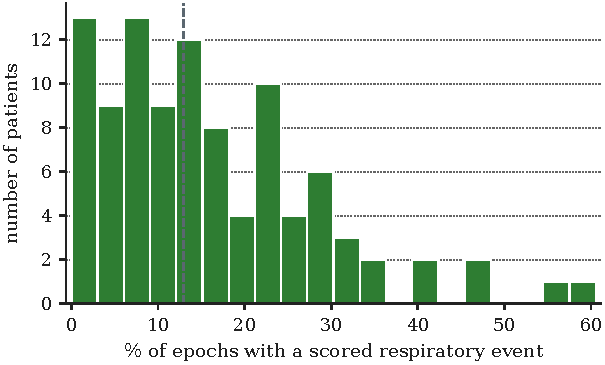
\includegraphics[width=0.62\textwidth]{figures/fig_mm_apnea_prev.pdf}
\caption{Patient-level respiratory-event burden in iSLEEPS, measured as the
fraction of 30-s epochs containing the onset of a scored respiratory event. The dashed line
denotes the cohort median of $13\%$.}
\label{fig:prev}
\end{figure}

\subsection{Sleep-EDF: Healthy-Sleep Reference Cohort}

Sleep-EDF is used to provide a healthy-sleep reference
~\cite{kemp2000sleepedf,goldberger2000physionet}. The experiments use the
Sleep Cassette subset corresponding to subjects 0--20, comprising 40 overnight
recordings. Because individual subjects can contribute more than one night,
splits are constructed at the subject level.

Sleep-EDF serves three purposes in this study. First, it provides an independent
check of the reimplemented sleep-staging architectures against the healthy-sleep
setting in which those models were originally evaluated. Second, models trained
on Sleep-EDF are applied to iSLEEPS without adaptation to examine transfer from
healthy sleep to the stroke cohort. Third, the proposed staging model is
evaluated on Sleep-EDF as an independent healthy-sleep cohort. The database
provides frontal EEG derivations including Fpz-Cz and Pz-Oz. It does not provide
the full cardiorespiratory signal set required by the proposed respiratory
branch and contains no respiratory-event annotations used by this study;
consequently, respiratory performance is not evaluated on Sleep-EDF.

\subsection{ISRUC-Sleep: Independent Sleep-Disorder Cohort}

ISRUC-Sleep provides the independent evaluation in populations with and without
sleep disorders~\cite{khalighi2016isruc}. Subgroup I contains $100$ patients with
sleep disorders recorded on one night each, subgroup II eight patients recorded
on two nights each, and subgroup III ten healthy adults. The recordings include
central and occipital EEG derivations corresponding to C4, C3, O2, and O1
referenced to the contralateral mastoid, two EOG derivations and chin EMG,
together with oronasal airflow, nasal pressure, thoracic and abdominal effort,
SpO$_2$, and ECG, and annotations of obstructive, central, and mixed apneas and
hypopneas; the annotations of the first scorer are used. Summed effort is formed
as the sum of the thoracic and abdominal traces, and pulse as the beat-to-beat
heart rate derived from ECG R-peaks, so that every iSLEEPS input has an ISRUC
counterpart. In $30$ of the $126$ ISRUC recordings the EDF header declares the
EEG and EOG range as $\pm25\,\mu$V, which places their N3 peak-to-peak amplitude
at $9$--$23\,\mu$V against $98$--$283\,\mu$V in the remaining recordings and below
the $75\,\mu$V that defines N3; these channels are restored by a factor of ten, a
correction decided from the header alone. One subgroup-I recording stores
monopolar EEG and EOG, from which the mastoid-referenced derivations are formed.

ISRUC-Sleep therefore supports evaluation of every output of the proposed
framework: sleep-stage prediction, respiratory-event prediction and, in subgroup I,
AHI estimation across the full severity range.

\subsection{UCD: Independent Sleep-Apnea Cohort}

The UCD database~\cite{ucddb2007,goldberger2000physionet} contains overnight PSG
from $25$ adults referred for suspected sleep-disordered breathing, with annotated
AHI between $1.2$ and $81.2$ events/h. It records C3 and C4 EEG only, which also
supply the occipital inputs, two EOG channels, chin EMG, ECG, oronasal airflow,
thoracic, abdominal and summed effort, SpO$_2$ and pulse, and its scored apneas
and hypopneas carry onset times. The EDF headers of this database carry no physical
unit, so EEG, EOG and EMG are scaled per recording to the median whole-night
amplitude of iSLEEPS, using no labels. UCD is used only for transfer.

\subsection{Signal Selection and Harmonization}

The iSLEEPS recordings contain 22 physiological and auxiliary traces. Fifteen
signals are retained for modeling and divided into neural and
cardiorespiratory groups. The neural group contains four EEG derivations
(C4:M1, C3:M2, O2:M1, and O1:M2), two EOG derivations (E1:M2 and E2:M2), and
the submental EMG. The cardiorespiratory group contains ECG, oronasal thermal
airflow, nasal pressure, thoracic effort, abdominal effort, summed respiratory
effort, SpO$_2$, and pulse.

Signals associated with periodic limb movement, snoring, plethysmography, body
position, ambient light, and device operation are not included in the model.
The snore channel is additionally excluded from respiratory prediction because
it is closely related to the airway information used during respiratory-event
assessment. Twelve iSLEEPS recordings lack at least one selected
cardiorespiratory channel. These patients are retained, and unavailable inputs
are zero-filled. The same
convention is used when a selected signal is unavailable in an external
dataset.

The datasets differ in montage and in the availability of
cardiorespiratory channels. Dataset-specific signal availability is therefore preserved, and external recordings are represented according to their available channels without assuming the complete iSLEEPS montage. Sleep-EDF is used only for analyses supported by its available sleep-staging signals, whereas ISRUC-Sleep provides sufficient
respiratory information to evaluate the respiratory output with unavailable inputs explicitly represented as missing channels.

\subsection{Preprocessing and Epoch Labels}

All sleep-stage predictions are defined on 30-s epochs. For iSLEEPS and
ISRUC-Sleep, the respiratory annotations are mapped to the same epoch grid. An
epoch is assigned a positive respiratory label if a scored respiratory event begins
within it and a negative label otherwise. The primary
respiratory task is therefore prediction of respiratory-event onset within
a 30-s epoch, and the patient-level AHI is derived from these predictions
(Section~\ref{sec:ahimethod}).

iSLEEPS retains only the epochs scored as a sleep stage, so a recording whose
hypnogram contains unscored rows has fewer retained epochs than $30$-s slots on
the recording clock. Every cardiorespiratory signal and every respiratory-event
label is therefore cut at the true recording time of each retained epoch. Cutting
them on the clock grid instead would shift them against the EEG after the first
unscored row; in iSLEEPS this concerns $63$ of the $100$ released recordings, by up
to $137$ epochs. The annotated AHI is the number of apneas and hypopneas starting
in scored sleep per hour of scored sleep.

For the iSLEEPS neural representation, the selected EEG, EOG, and EMG signals
are resampled to $100$\,Hz for computation of the engineered descriptors
described in Section~\ref{sec:features}. The LaBraM encoder receives the four
EEG derivations and the two EOG derivations. Because LaBraM was pretrained at
$200$\,Hz, these signals are independently resampled to $200$\,Hz before entering
the encoder. The EMG channel is not supplied to LaBraM.

The eight cardiorespiratory inputs are resampled to a common $25$\,Hz grid
using polyphase resampling before entering the learned cardiorespiratory
encoder. SpO$_2$ is recorded natively at $4$\,Hz and is placed on the same
$25$\,Hz grid for temporal alignment with the remaining channels; this
operation does not increase the underlying temporal resolution of the
oximeter signal. Raw cardiorespiratory signals remain in their recorded
physical units after resampling.

Engineered feature representations are standardized within each recording
before model input. For iSLEEPS, where each analyzed patient contributes one
overnight recording, this corresponds to the patient-wise standardization used
throughout the primary analysis. The same per-recording procedure is applied
when the trained model is evaluated on the external datasets. No labels from an
external dataset are used to refit model parameters, select thresholds, or
adapt the reported iSLEEPS model.

%=====================================================================
\section{Proposed Method}
\label{sec:method}
\subsection{Problem Formulation}
A night is a sequence of $T$ epochs. For epoch $t$ we form a neural feature vector
$\mathbf{f}^{\mathrm{eeg}}_t\in\mathbb{R}^{388}$, formed by concatenating the $188$
engineered descriptors below with a $200$-dimensional embedding from LaBraM, a
pretrained EEG encoder~\cite{labram2024} adapted to sleep (Section~\ref{sec:encoder}), and a raw cardiorespiratory tensor
$\mathbf{x}^{\mathrm{car}}_t\in\mathbb{R}^{8\times750}$, the eight channels at $25$\,Hz.
The $14$ engineered cardiorespiratory descriptors defined below are used by the baseline
configuration against which the learned encoder is measured.

The pretrained encoder is supplied with input in the format used during its pretraining. LaBraM was
pretrained at $200$\,Hz and fixes its input length at $3000$ samples, so the EEG is
resampled from our $100$\,Hz working rate to $200$\,Hz before it reaches the encoder.
Supplying the $100$\,Hz signal directly would introduce an undetected error: $3000$ samples would then span $30$\,s of recording while the encoder interprets them as $15$\,s, compressing time by a factor of two, so that every rhythm would appear at twice its frequency and a $12$\,Hz spindle at $24$\,Hz. At $200$\,Hz a $30$\,s epoch no longer fits the positional embedding in one piece, so each epoch is split into two $15$\,s sub-windows of $3000$ samples, encoded separately, and mean-pooled; the two embeddings were verified to differ before caching, so the pooling combines distinct information from the two sub-windows. The encoder also requires canonical $10$--$20$ names
and rejects mastoid references, so C4:M1, C3:M2, O2:M1 and O1:M2 are presented as C4,
C3, O2 and O1. The two EOG derivations are presented as F7 and F8, the frontal
positions nearest the eyes, so that the encoder receives the ocular activity that
separates REM from Wake; the chin channel is not supplied. Amplitudes are scaled to
$\mu$V$/100$. The encoder therefore sees four EEG and two EOG channels. We learn a subject-independent
map
\begin{equation}
f_\theta:\big(\mathbf{f}^{\mathrm{eeg}}_{1:T},\mathbf{x}^{\mathrm{car}}_{1:T}\big)\ \longmapsto\
\big(\hat y^{\mathrm{stg}}_{1:T},\ \hat y^{\mathrm{apn}}_{1:T}\big),
\end{equation}
where $\Delta^4=\{p\in\mathbb{R}^5:p_k\geq 0,\ \sum_k p_k=1\}$ is the four-simplex,
$\hat y^{\mathrm{stg}}_t\in\Delta^4$ is a distribution over the five stages and
$\hat y^{\mathrm{apn}}_t\in[0,1]$ scores whether epoch $t$ contains a respiratory
event (Figure~\ref{fig:arch}). We write $\hat y^{\mathrm{apn}}_t$ as a score and not as a
probability for the reason given in Section~\ref{sec:training}: the positive weighting in its
loss displaces the optimum away from the conditional event rate.

\begin{figure}[pos=H]
\centering
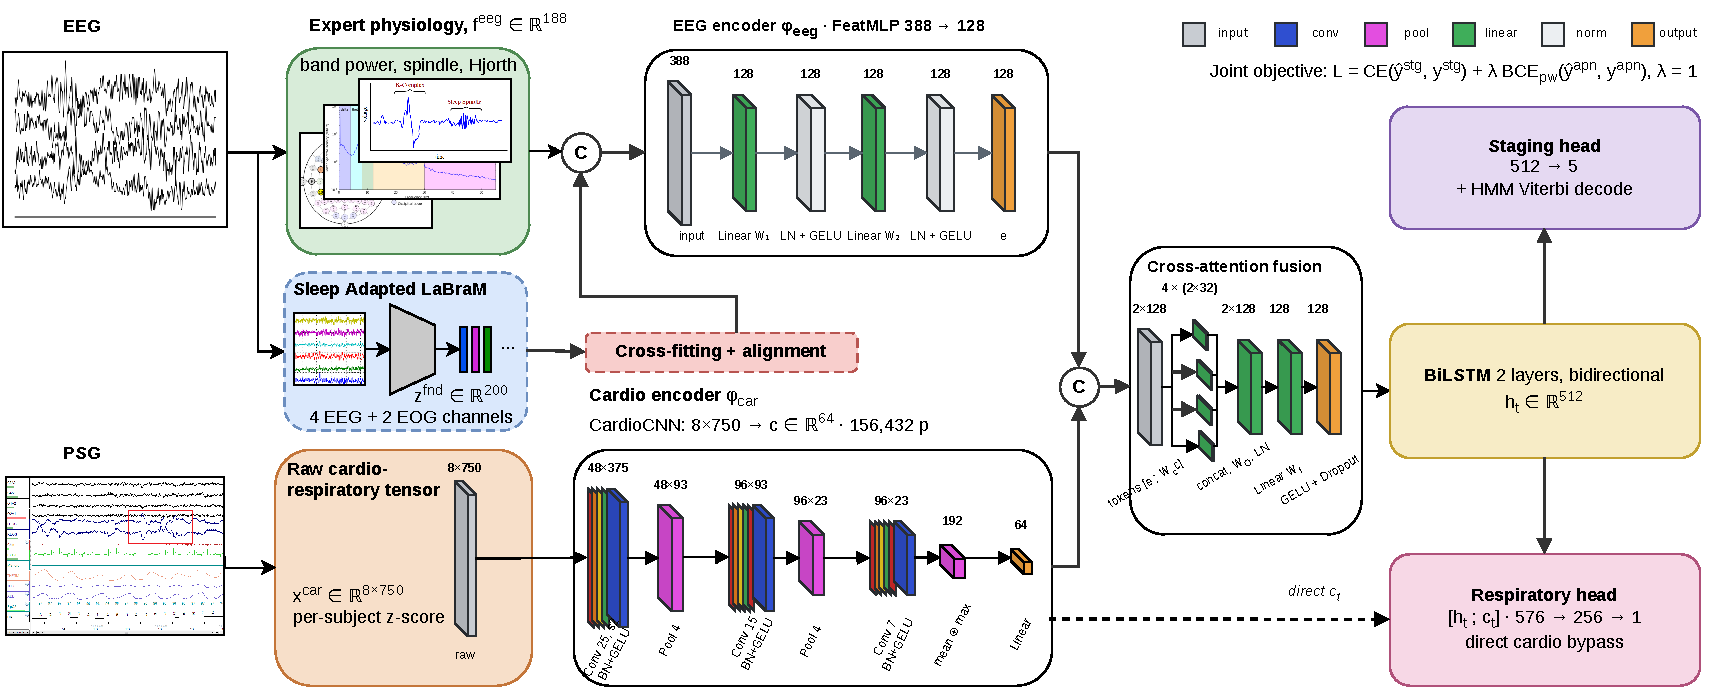
\includegraphics[width=\textwidth, height=7cm]{figures/fig_architecture.pdf}
\caption{The two-stream, multi-task model. The neural stream combines $188$ engineered
descriptors with the embedding of a LaBraM encoder adapted to sleep from EEG and EOG and
integrated by cross-fitting and alignment; the cardiorespiratory stream is a convolutional
encoder over eight raw channels. The streams are fused and read by a bidirectional LSTM over
a $20$-epoch window, which feeds a staging head and a respiratory head; the respiratory head
also reads the cardiorespiratory embedding directly, and the AHI is computed from the
respiratory scores over decoded sleep.}
\label{fig:arch}
\end{figure}

\subsection{Physiological Feature Representations}
\label{sec:features}
\paragraph{Neural features ($188$)}
Per channel we take absolute and relative band powers from the Welch spectrum $P(f)$ in delta
($0.5$--$4$), theta ($4$--$8$), alpha ($8$--$13$), sigma ($11$--$16$), and beta
($16$--$30$)\,Hz; the relative power in band $b$ is
\begin{equation}
\mathrm{RP}_b=\frac{\int_{f\in b}P(f)\,df}{\int_{0.5}^{30}P(f)\,df}.
\end{equation}
The bands are the conventional sleep bands and alpha and sigma overlap between $11$ and
$13$\,Hz, so the five relative powers are not a partition and do not sum to one. We retain the conventional definitions because both bands correspond to physiology assessed in visual scoring, and the model treats the five values as correlated descriptors whose sum is unconstrained.
We add spectral entropy $H=-\sum_i p_i\log p_i$ with $p_i$ the normalized spectrum, the
$95\%$ spectral-edge frequency, the three Hjorth descriptors~\cite{hjorth1970eeg}, and
time-domain statistics. Sleep spindles are detected on the sigma-band analytic envelope,
the modulus of the analytic signal built from the Hilbert transform $\mathcal{H}$,
$e(t)=\lvert x_\sigma(t)+i\,\mathcal{H}\{x_\sigma\}(t)\rvert=\sqrt{x_\sigma(t)^2+\mathcal{H}\{x_\sigma\}(t)^2}$, with
density counted above a per-epoch threshold. No duration, separation or morphology criterion is applied, so this measure counts crossings of a sigma-band envelope and serves as a proxy for spindle density; it is not a validated spindle detector. The slow-wave descriptors likewise summarise slow-wave amplitude without detecting discrete waves. Ocular-movement energy on
the EOG and tonic EMG level complete the set.

\paragraph{Cardiorespiratory features ($14$)}
From the seven cardiorespiratory channels we compute SpO$_2$ mean, minimum, variability, and
desaturation depth (median minus minimum); pulse mean and variability; ECG amplitude and
line-length; airflow amplitude and line-length; thoracic, abdominal, and summed effort
amplitudes; and signed thoraco-abdominal synchrony, whose loss is the paradoxical motion of
chest against abdomen that marks an obstructed breath. The correlation is kept signed, so
synchronous and paradoxical motion sit at opposite ends of the range; a value near $+1$ is synchronous motion and a negative value is paradox,
\begin{equation}
\mathrm{sync}_t=\mathrm{corr}(x^{\mathrm{tho}}_t,\ x^{\mathrm{abd}}_t).
\end{equation}
Both feature sets are standardized per patient, which removes person-to-person offsets and reduces the sensitivity of the model to inter-individual differences.

\paragraph{The learned cardiorespiratory encoder}
The evaluated model does not read the $14$ descriptors. Its cardiorespiratory branch is a three-layer convolutional encoder over the raw $8\times750$ tensor, with wide kernels and aggressive downsampling because respiratory events are slow: at $25$\,Hz the first kernel of $25$ samples spans one second, and a hypopnea unfolds over $10$ to $30$\,s. Channel widths are
$48$, $96$ and $96$, each followed by batch normalisation and GELU, with max-pooling by four
after the first two. Mean and max pooling over time are concatenated and projected by a
linear layer, LayerNorm, GELU and dropout to the same
$64$ dimensions as the cardiorespiratory feature MLP it replaces, so the encoder is a drop-in replacement and every
other part of the network is unchanged. The branch holds about $0.16$\,M trainable
parameters ($155{,}232$ in the seven-channel configuration). Section~\ref{sec:repr} quantifies the effect of this substitution, which is among the largest representation changes we measure, and Section~\ref{sec:nested} shows that the effect is attributable to the change of representation: random encoders of comparable capacity over the same raw signal recover much of it. This encoder is used because it is small,
trained end-to-end with the rest of the network, and adds no external dependency.

\subsection{Sleep-Adapted EEG Encoder}
\label{sec:encoder}
\paragraph{Adaptation} Within each training fold, LaBraM-Base ($5.8$\,M parameters) is
fine-tuned with a linear staging head on single epochs of the fold's training patients, using
AdamW at $3\times10^{-5}$ for the encoder and $10^{-3}$ for the head, a one-cycle schedule
over three passes of the training epochs, batch size $64$ and mixed precision; the state with
the highest accuracy on the fold's validation patients is kept. Test patients never reach the
encoder.

\paragraph{Cross-fitting} An encoder fine-tuned on a patient embeds that patient in-sample. If the downstream model is trained on such embeddings and tested on out-of-sample ones, the two distributions differ, and the downstream model is fitted to representations of higher quality than those available at test time. Each fold's training patients are therefore split
into $K=3$ parts $P_1,P_2,P_3$, and an encoder $\phi_k$ is fine-tuned on the training patients
outside $P_k$; every training patient in $P_k$ is embedded by $\phi_k$, an encoder that never
saw it. The full-fold encoder $\phi$, fine-tuned on all training patients, embeds the
validation and test patients.

\paragraph{Alignment} Cross-fitting makes every embedding out of sample but places the
training patients in the spaces of $K$ different encoders, which do not coincide with the
space of $\phi$ used at test time. Each $\phi_k$ is mapped into the space of $\phi$ by a ridge
regression~\cite{hoerl1970ridge} fitted on the patients of $P_k$, for whom both embeddings
exist,
\begin{equation}
W_k=\arg\min_W\big\lVert(E^{\phi}_{P_k}-\mu^{\phi}_k)-(E^{\phi_k}_{P_k}-\mu^{\phi_k}_k)W\big\rVert_F^2
+\lambda n_k\lVert W\rVert_F^2,
\end{equation}
and the training embeddings become
$\tilde{\mathbf{e}}_t=(\mathbf{e}^{\phi_k}_t-\mu^{\phi_k}_k)W_k+\mu^{\phi}_k$, with $\lambda=0.01$
and $n_k$ the number of epochs in $P_k$. The map uses training patients only. Every training
embedding is thereby out of sample and expressed in the coordinates the downstream model
receives at test time; Section~\ref{sec:integration} shows that both properties are
required.

\subsection{Two-Stream Encoders}
The neural stream is a two-layer perceptron with LayerNorm; the cardiorespiratory stream is the convolutional encoder described above, which emits a vector of the same width as the feature perceptron it replaced,
\begin{align}
e_t&=\mathrm{GELU}\!\big(\mathrm{LN}(W_2\,\mathrm{GELU}(\mathrm{LN}(W_1\mathbf{f}^{\mathrm{eeg}}_t))) \big)\in\mathbb{R}^{128},\\
c_t&=\mathrm{CardioCNN}\big(\mathbf{x}^{\mathrm{car}}_t\big)\in\mathbb{R}^{64}.
\end{align}
LayerNorm is used in place of BatchNorm because the recurrent windows are short and mix patients within a batch, and the cardiorespiratory stream is deliberately narrower because the branch compresses an $8\times750$ tensor into the same $64$ dimensions as the feature encoder it replaced, so that the substitution is the only variable.

\subsection{Fusion}
Two fusion operators are used. Concatenation projects the joined embeddings back to the
stream width,
\begin{equation}
z_t=\mathrm{GELU}\!\big(W_f\,[\,e_t\ ;\ c_t\,]\big)\in\mathbb{R}^{D},\qquad D=128.
\end{equation}
Cross-attention treats the two embeddings as tokens carrying learned modality-type
embeddings, refines them by four-head scaled dot-product attention so that each modality
reads the other, and projects the result to $z_t\in\mathbb{R}^{D}$. In the feature-only
configuration the two were indistinguishable on staging ($+0.005$ accuracy, $p=0.49$) and
concatenation was slightly ahead on the respiratory head ($0.014$ AUC, $p=0.06$), so the
controlled analyses below use concatenation. With uniform class weights and the
sleep-adapted encoder, cross-attention was carried forward on validation accuracy and is the
fusion of the final MM-Net (Table~\ref{tab:components}).

\subsection{Temporal Decoder and Two Heads}
Sleep is sequential and respiratory events cluster, so the fused vectors of an $L=20$ epoch
window ($10$ minutes) are read by a two-layer bidirectional LSTM. Training draws windows at a stride of $L/2$, so an interior epoch is seen twice per pass and an epoch in the first or last ten of a recording once; no correction is applied for this imbalance, and the first and last window of each night are zero-padded to $L$ under a mask that removes the padding from the loss.
Inference uses disjoint windows: a recording is padded to a multiple of $L$, split into
consecutive blocks, and the padding discarded, so every epoch is scored exactly once and no
stitching rule is needed. Hidden states are not carried between windows in either case.
Each direction runs the
standard recurrence
\begin{align}
i_t&=\sigma(W_i[z_t,h_{t-1}]), & f_t&=\sigma(W_f[z_t,h_{t-1}]),\nonumber\\
o_t&=\sigma(W_o[z_t,h_{t-1}]), & g_t&=\tanh(W_g[z_t,h_{t-1}]),\\
s_t&=f_t\odot s_{t-1}+i_t\odot g_t, & h_t&=o_t\odot\tanh(s_t),\nonumber
\end{align}
and the forward and backward states of the $256$-unit layers are concatenated into
$h_t\in\mathbb{R}^{512}$. The
staging head is a linear map $\hat y^{\mathrm{stg}}_t=\mathrm{softmax}(W_s h_t)$. The
respiratory head reads $h_t$ together with a direct copy of the per-epoch cardiorespiratory
embedding $c_t$,
\begin{equation}
\hat y^{\mathrm{apn}}_t=\sigma\!\big(W_2\,\mathrm{GELU}(W_1[h_t;c_t])\big).
\end{equation}

The respiratory head receives the per-epoch cardiorespiratory embedding $c_t$
directly in addition to the shared temporal representation. In the frozen-encoder
configuration (Section~\ref{sec:results}), removing this bypass
reduces respiratory AUC from $\fzAuc$ to $0.776$ ($p=0.049$) and average
precision from $\fzAp$ to $0.411$ ($p=0.28$), while staging remains unchanged
at $0.739$ accuracy and $\kappa=0.634$ ($p=0.92$ for both). The ablation
preserves the parameter count by zeroing. A control that permutes the same embeddings across
epochs, preserving their distribution while disrupting temporal alignment,
reaches $0.774$ AUC. These results indicate a modest task-specific contribution
from temporally aligned cardiorespiratory information at the respiratory head.


MM-Net holds $2.85$ million trainable parameters. The sleep-adapted encoder that supplies
the $200$-dimensional neural embedding ($5.8$ million parameters) is fine-tuned in a separate
stage per fold (Section~\ref{sec:encoder}) and run once to cache the embeddings, so it is not
part of this count.

\subsection{Training and Decoding}
\label{sec:training}
The two tasks are trained together with equal weight, $\mathcal{L}=\mathcal{L}^{\mathrm{stg}}+\lambda\,\mathcal{L}^{\mathrm{apn}}$ with $\lambda=1$, combining a class-weighted staging cross-entropy and a positive-weighted respiratory cross-entropy,
\begin{align}
\mathcal{L}^{\mathrm{stg}}&=-\sum_t\sum_{k}w_k\,y^{\mathrm{stg}}_{t,k}\log\hat y^{\mathrm{stg}}_{t,k},\\
\mathcal{L}^{\mathrm{apn}}&=-\sum_t\big[\pi\,a_t\log\hat y^{\mathrm{apn}}_t+(1-a_t)\log(1-\hat y^{\mathrm{apn}}_t)\big].
\end{align}
The final MM-Net uses uniform staging weights ($w_k=1$), selected on validation patients
together with the encoder (Table~\ref{tab:components}); the controlled analyses use the
square root of inverse class frequency,
$w_k\propto\sqrt{N/(K n_k)}$ for $K=5$ classes with $n_k$ examples, which corrects the scarce
N1 and N3 stages. In both, the respiratory term is
positive-weighted by $\pi=n_-/n_+$ to match the $16\%$ event rate, which on this corpus is
$\pi\approx5.3$.

Both weightings shift the optimum of the loss, as follows. Against a true conditional rate $p$, the weighted binary term attains its minimum at $q^{\star}=\pi p/[\pi p+(1-p)]$, which exceeds $p$ whenever $\pi>1$, so an epoch carrying a true event probability of $0.160$ is driven towards $0.5$; the staging weights displace the softmax by the same mechanism, to $q^{\star}_k\propto w_k p_k$. Neither head therefore emits a calibrated posterior, and a
threshold of $0.5$ on the respiratory output is not a fifty-per-cent event probability. Both displacements are monotone, so ranking is unaffected and the AUC and average precision we report are unchanged; the displacements affect only the interpretation of the outputs as probabilities, so the outputs are treated as scores and calibration is assessed separately (Section~\ref{sec:results}).

At inference the staging
posteriors are smoothed by a Viterbi pass whose transition matrix $A^{\mathrm H}$
and prior are counted from the training labels~\cite{chen2024hmm},
\begin{equation}
\delta_t(j)=\max_i\big[\delta_{t-1}(i)+\log A^{\mathrm H}_{ij}\big]+\log\hat y^{\mathrm{stg}}_t(j),
\end{equation}
recovered by back-tracking, which restores the natural persistence of sleep.

This is a transition-regularised discriminative decoder and not a generative hidden Markov
model. A generative emission term is
$\log P(\mathbf{x}_t\mid s_t=j)$, whereas $\hat y^{\mathrm{stg}}_t(j)$ is a class-weighted
discriminative score computed from a bidirectional window; inserting it in the emission slot
applies the stage prior a second time, once through $A^{\mathrm H}$ and once through the
score itself. Dividing by the prior would not repair this, because the class weights and the recurrent context have already displaced the score from a calibrated posterior.
The pass therefore functions as a transition prior on the output sequence. The respiratory
head is left unsmoothed. Optimization uses AdamW with cosine annealing and early stopping on a
held-out set of patients. Three seeds are trained per fold, and the final MM-Net is reported
both as a single model (the mean over seeds) and as the three-seed average of the softmax
outputs.

\subsection{AHI Estimation}
\label{sec:ahimethod}
Because $\hat y^{\mathrm{apn}}_t$ scores event onsets, its sum over the epochs decoded as sleep
estimates the number of events, and dividing by the decoded sleep time gives a rate,
\begin{equation}
\widehat{\mathrm{AHI}}=k\cdot\frac{\sum_{t:\hat s_t\neq\mathrm{W}}\hat y^{\mathrm{apn}}_t}{\tfrac{30}{3600}\,\lvert\{t:\hat s_t\neq\mathrm{W}\}\rvert}.
\end{equation}
The positive weighting of the respiratory loss inflates the scores
(Section~\ref{sec:training}), so a single scale $k$ is fitted in each fold as the median ratio
of annotated to raw estimate over the fold's validation patients and applied unchanged to its
test patients. For transfer to another cohort, $k$ is the median of the ten iSLEEPS fold
values ($0.459$), and nothing is refitted on the external cohort. Severity follows the AASM
bands ($<5$, $5$--$15$, $15$--$30$ and $\geq30$ events/h).

%=====================================================================
\section{Experiments}
\label{sec:results}
\subsection{Protocol and Metrics}
All results use ten-fold, patient-independent cross-validation, so no patient appears in both
training and test, and within each training split a disjoint set of patients is held out for
early stopping. Staging is scored by accuracy, macro-F1 $\tfrac{1}{K}\sum_k\mathrm{F1}_k$, and
Cohen's $\kappa$. The respiratory task is scored by the area under the ROC curve (AUC) and
average precision (AP), which suits the $16\%$ event rate, and the AHI estimate by Spearman's
$\rho$, the mean absolute error (MAE), severity-band accuracy and linearly weighted $\kappa$.

Two configurations of the same architecture are reported. The final MM-Net uses the
sleep-adapted, cross-fitted and aligned encoder, eight cardiorespiratory channels,
cross-attention fusion and uniform staging weights; it produces every headline result. The
controlled analyses (respiratory bypass, fusion, modality ablation, joint objective, incomplete
montage, permutation importance, stream representations, loss constants,
calibration and nested selection) use the frozen-encoder configuration, which shares the
streams, decoder and heads but reads a frozen LaBraM embedding of the EEG, seven
cardiorespiratory channels, concatenation fusion and square-root class weights. Each of those
analyses retrains dozens of variants, and adapting the encoder anew for every variant would
multiply their cost by the four encoder trainings each fold requires. The frozen-encoder
configuration reaches $\fzAcc$ accuracy ($\kappa$ $\fzK$) and $\fzAuc$ respiratory AUC, and the
quantities it is used to establish concern the streams, the objective and the
representations that both configurations share.

Every number we report is a mean over the ten folds with its standard deviation. This standard deviation describes dispersion across folds and is not a confidence interval; because the folds share training patients, they are dependent. Because patients are approximately independent units, we also resample patients with replacement, $10{,}000$ times, rebuilding the pooled epoch set and recomputing every metric. For the
frozen-encoder configuration this gives $0.734$ accuracy with a $95\%$ interval of $[0.717,\ 0.750]$, $\kappa$ $0.628$
$[0.604,\ 0.651]$, respiratory AUC $0.778$ $[0.752,\ 0.802]$ and average precision $0.419$
$[0.355,\ 0.480]$. These intervals are conditional on the fitted procedure: they reflect variation across the recorded patients but exclude retraining variability and the selection optimism quantified below. The
folds are fixed across all configurations so that comparisons are paired. Fixed folds introduce a potential selection effect, quantified below: the frozen-encoder configuration was chosen by comparing forty-nine candidates on these same ten folds, which can introduce selection optimism into in-domain estimates. This optimism was measured by repeating the selection with the test patients held out from model selection (Section~\ref{sec:nested}): five outer patient-independent folds, all forty-nine candidates compared on three inner folds within each outer training set, and the winner scored once on outer patients that took no part in choosing it. That procedure reaches $0.734 \pm 0.009$ accuracy against its $\fzAcc$, so the optimism is $0.006$, about a third of the fold-to-fold standard deviation of $0.019$, and it does not alter any comparison reported here. The external corpora in Section~\ref{sec:external} took no part in selection either, so the transfer results reported there are not subject to this selection effect. The proposed
model, its ablations and the retrained baselines all use the full ten; only the Sleep-EDF
transfer row was run at five, as stated in the discussion of Table~\ref{tab:bench}. Because performance estimates may vary
across random seeds, we retrained the frozen-encoder configuration under three
seeds on the same folds. Staging accuracy varies by $0.005$ across seeds against
$0.020$ across folds, and respiratory AUC by $0.001$ against $0.038$: fold-to-fold spread
is four times the seed spread for staging and about thirty-four times it for respiratory detection.
The uncertainty in these results is therefore dominated by which patients fall in which
fold, which is a property of a cohort this size. Every headline figure in this paper is the mean over all thirty fold-values, ten
folds by three seeds. Paired tests, however, are computed on the ten fold-means: the three seeds within a fold train and test on the same patients, so they constitute repeated training runs on one patient partition, and treating them as thirty independent observations would inflate the effective sample size threefold and understate every $p$-value. Consequently, with ten paired folds the smallest two-sided Wilcoxon $p$ is $2/2^{10}=0.002$, reached when every fold moves the same way, so after Holm correction across a family of nine the floor is $0.018$. Several effects below sit at that floor and differ in size by more than an order of
magnitude; the test cannot separate them, and the effect sizes are reported beside every
$p$ for that reason. The comparisons of the respiratory bypass, the joint objective, the fusion
type and the incomplete-montage subgroups are secondary analyses and are reported without
multiplicity correction. The three seed means for respiratory AUC are
$0.781$, $0.783$ and $0.781$, so $\fzAuc$ is stable to the third decimal under reseeding.

\subsection{Selection Inside the Training Data}
\label{sec:nested}
The frozen-encoder configuration was chosen on the folds that score it; the encoder, fusion and
class weights of the final MM-Net were chosen on validation patients only. To quantify the contribution of this selection, the entire selection was repeated with the test patients held out from model selection: five outer patient-independent folds; inside each outer training set, three inner folds; all forty-nine candidates of the original search compared on those inner folds alone; and the inner winner retrained on the full outer training set and scored once on the outer patients.
No outer patient influences the choice of the model that scores them, so the resulting estimate covers the complete procedure, including the search.

The nested procedure yields a comparable estimate, reaching $0.7336 \pm 0.0089$ accuracy across the five outer folds against $\fzAcc$ for the frozen-encoder configuration. The estimated selection optimism is therefore $0.006$ accuracy, about a third of the
fold-to-fold standard
deviation and smaller than the performance differences underlying the principal comparisons.
It is also close to the $0.004$ suggested by the spread of the top ten candidates, indicating that the estimate available without a nested loop was of the correct order of magnitude.

Across the five outer folds, the neural configuration is selected consistently. The engineered descriptors, frozen pretrained encoder, BiLSTM, width, and
regularisation are retained. The cardiorespiratory representation varies across
folds: four select a randomly initialised time-series encoder over the raw signal,
while one selects a random projection of the fourteen engineered descriptors;
none selects the learned convolutional encoder.

Together with the representation experiments in Section~\ref{sec:repr}, this indicates that richer cardiorespiratory representations are useful and that no single encoder architecture is consistently preferred at this cohort size.
The selected configurations remain within $0.006$ staging accuracy of the frozen-encoder configuration.

Because each outer model is trained jointly, the nested procedure also provides a
selection-free estimate for the respiratory output. Across the five outer folds, respiratory AUC is $0.774 \pm 0.047$ and average precision is $0.406 \pm 0.077$, corresponding to differences of $0.008$ AUC and $0.013$ average precision relative to the frozen-encoder configuration.
These differences are similar in scale to the staging selection effect and are small relative
to the respiratory fold-to-fold standard deviation of $0.038$. The inner loop selects models
using staging accuracy. The four outer folds selecting the randomly initialised time-series
encoder average $0.793$ respiratory AUC; the remaining fold, which selected the random
projection of the fourteen descriptors, yields $0.698$. The nested estimate therefore
remains above the $0.698$ obtained with the fourteen engineered descriptors in the same
configuration (Table~\ref{tab:repr}).

The nested estimate uses five outer folds and a single training seed and is therefore less precise than the ten-fold, three-seed headline evaluation.

\subsection{Implementation and Hyperparameters}
The model is implemented in PyTorch and trained on single NVIDIA RTX~2060 (6\,GB) and
RTX~3060\,Ti (8\,GB) GPUs under Windows. Every run is seeded, so each is individually reproducible; headline figures
average three seeds ($42$, $1$, $7$) over the ten folds, giving the thirty fold-values used
throughout. Where a result is derived from stored predictions without retraining, it comes from the seed-$42$ run, and this is stated where it applies.
Table~\ref{tab:hyper} lists the training configuration, which is identical across all folds and every ablation, so that reported differences reflect the model configuration. The six reimplemented baselines are trained at the optimiser, batch size and schedule of their own papers, because imposing our settings could disadvantage architectures tuned for other settings.

\begin{table}[H]
\caption{Training configuration of the final MM-Net, shared across all folds and cohorts. The
controlled analyses use the same settings with a frozen encoder, concatenation and square-root
class weights. Each reimplemented baseline is trained at its own published settings.}
\label{tab:hyper}
\centering
\small
\adjustbox{max width=\textwidth}{%
\begin{tabular}{ll}
\toprule
Setting & Value \\
\midrule
Framework / hardware & PyTorch, NVIDIA RTX~2060 / 3060\,Ti \\
\multicolumn{2}{@{}l}{\emph{Sleep-adapted encoder (per fold)}} \\
Encoder & LaBraM-Base, $4$ EEG $+$ $2$ EOG \\
Encoder LR (head) & $3\times10^{-5}$ ($10^{-3}$), one-cycle \\
Passes, batch, weight decay & $3$, $64$, $0.05$ \\
Cross-fitting, alignment & $K=3$, ridge $\lambda=0.01$ \\
\multicolumn{2}{@{}l}{\emph{MM-Net}} \\
Optimizer & AdamW \\
Learning rate & $3\times10^{-4}$ \\
Weight decay & $1\times10^{-4}$ \\
LR schedule & cosine annealing \\
Sequence length $L$ & $20$ epochs ($10$\,min) \\
Batch size & $32$ \\
Max epochs / patience & $45$ / $8$ \\
Gradient clipping & $5.0$ \\
Fusion & cross-attention, $4$ heads \\
Staging class weights & uniform \\
Respiratory pos.\ weight & $\pi=n_-/n_+$ \\
Loss balance $\lambda$ & $1.0$ \\
Staging post-processing & HMM Viterbi smoothing \\
Cross-validation & $10$-fold, patient-independent \\
Random seeds & $42$, $1$, $7$ \\
\bottomrule
\end{tabular}}
\end{table}

\subsection{Compared Methods}
We compare the model against deep networks evaluated on the same folds: convolutional and
recurrent networks trained from scratch (DeepSleepNet, AttnSleep, a four-channel CNN--BiLSTM),
six further published architectures we reimplemented for this comparison (U-Time, a
fully convolutional encoder--decoder; TinySleepNet, a compact convolutional--recurrent model;
SleepTransformer, a purely attentional one; and 1D-ResNet-SE-LSTM, Micro SleepNet and
AT-BiLSTM), the released SE-ResNet-18 implementation from~\cite{bose2026gap}, a
network transferred from Sleep-EDF, and a raw-signal convolutional network on all $14$ channels,
alongside the published single-channel baselines for the corpus~\cite{maiti2026isleeps}. For the
respiratory task, a desaturation rule, logistic regression and gradient boosting read the $14$
engineered cardiorespiratory descriptors, and two raw-signal detectors read the waveforms
(Section~\ref{sec:noflow}). On ISRUC-I, the reimplemented staging baselines are retrained on
MM-Net's folds (Section~\ref{sec:external}). All numbers are
patient-independent. All use ten folds except the Sleep-EDF transfer row, which uses five; hidden-Markov decoding is applied where the corresponding model provides it.

\begin{table}[H]
\caption{Reimplementation checks on Sleep-EDF for the models marked $^{\dagger}$ in Table~\ref{tab:bench}. Published and reproduced values are compared under their respective reported protocols; U-Time is compared using macro-F1, while the remaining rows use accuracy.}
\label{tab:reimpl}
\centering
\begin{tabular}{@{}l c c c@{}}
\toprule
Model & Published & Reproduced & $\Delta$ \\
\midrule
U-Time~\cite{perslev2019utime}$^{\S}$ & 0.79 & $0.660 \pm 0.054$ & $-0.130$ \\
TinySleepNet~\cite{supratak2020tinysleepnet} & 0.854 & $0.824 \pm 0.045$ & $-0.030$ \\
SleepTransformer~\cite{sleeptransformer2022} & 0.814 & $0.823 \pm 0.033$ & $+0.009$ \\
1D-ResNet-SE-LSTM~\cite{li2023resnetselstm} & 0.864 & $0.832 \pm 0.036$ & $-0.032$ \\
Micro SleepNet~\cite{liu2023microsleepnet} & 0.828 & $0.800 \pm 0.041$ & $-0.028$ \\
AT-BiLSTM~\cite{fu2021atbilstm} & 0.838 & $0.835 \pm 0.046$ & $-0.003$ \\
\bottomrule
\end{tabular}
\end{table}

\begin{table}[H]
\caption{Patient-independent sleep-staging comparison on iSLEEPS. Values are mean $\pm$ SD where fold-level results are available. $^{\dagger}$ denotes reimplemented models, $^{\ddagger}$ a literature-reported result under its original protocol, and $^{\ast}$ models ported from released code. Bold indicates the best result among models evaluated under our protocol.}
\label{tab:bench}
\centering
\adjustbox{max width=\textwidth}{%
\begin{tabular}{@{}l l c c c c c@{}}
\toprule
 & & & Healthy & \multicolumn{3}{c}{iSLEEPS (stroke)} \\
\cmidrule(lr){4-4}\cmidrule(lr){5-7}
Model & Input & Params\,$\downarrow$ & Acc & Acc\,$\uparrow$ & Macro-F1\,$\uparrow$ & $\kappa$\,$\uparrow$ \\
\midrule
\multicolumn{7}{@{}l}{\emph{Comparative models evaluated on iSLEEPS}}\\[1pt]
LSTM, our reimplementation$^{\dagger}$ & 1\,EEG\,$+$\,EOG & $1.16$\,M & $0.820 \pm 0.062$ & $0.720 \pm 0.032$ & $0.626 \pm 0.028$ & $0.599 \pm 0.043$ \\
CNN-ResNet18~\cite{bose2026gap}$^{\ddagger}$ & 1\,EEG & $\sim$11\,M & --- & 0.617 & 0.544 & 0.480 \\
SE-ResNet-18\,+\,BiLSTM~\cite{bose2026gap}$^{\ast}$ & 1\,EEG & $11.32$\,M & $0.829 \pm 0.056$ & $0.696 \pm 0.038$ & $0.606 \pm 0.032$ & $0.572 \pm 0.046$ \\
DeepSleepNet~\cite{supratak2017deepsleepnet}  & 4\,EEG  & $3.72$\,M  & $0.823 \pm 0.050$ & $0.669 \pm 0.031$ & $0.624 \pm 0.026$ & $0.558 \pm 0.035$ \\
U-Time~\cite{perslev2019utime}$^{\dagger}$ & 1\,EEG & $1.07$\,M & $0.791 \pm 0.062$ & $0.646 \pm 0.064$ & $0.524 \pm 0.057$ & $0.506 \pm 0.082$ \\
AttnSleep~\cite{eldele2021attnsleep}          & 1\,EEG  & $\sim$0.5\,M & $0.833 \pm 0.042$ & $0.716 \pm 0.042$ & $0.600 \pm 0.043$ & $0.593 \pm 0.058$ \\
TinySleepNet~\cite{supratak2020tinysleepnet}$^{\dagger}$ & 1\,EEG & $1.45$\,M & $0.824 \pm 0.045$ & $0.676 \pm 0.050$ & $0.587 \pm 0.034$ & $0.548 \pm 0.062$ \\
SleepTransformer~\cite{sleeptransformer2022}$^{\dagger}$ & 1\,EEG & $2.79$\,M & $0.823 \pm 0.033$ & $0.683 \pm 0.026$ & $0.602 \pm 0.030$ & $0.555 \pm 0.032$ \\
1D-ResNet-SE-LSTM~\cite{li2023resnetselstm}$^{\dagger}$ & 1\,EEG & $0.65$\,M & $0.832 \pm 0.036$ & $0.708 \pm 0.038$ & $0.631 \pm 0.033$ & $0.592 \pm 0.050$ \\
Micro SleepNet~\cite{liu2023microsleepnet}$^{\dagger}$ & 1\,EEG & $0.03$\,M & $0.800 \pm 0.041$ & $0.647 \pm 0.049$ & $0.558 \pm 0.028$ & $0.510 \pm 0.055$ \\
AT-BiLSTM~\cite{fu2021atbilstm}$^{\dagger}$ & 1\,EEG & $0.92$\,M & $0.835 \pm 0.046$ & $0.692 \pm 0.040$ & $0.612 \pm 0.030$ & $0.570 \pm 0.051$ \\
CNN\,+\,BiLSTM                                & 4\,EEG  & $\sim$0.6\,M & $0.806 \pm 0.041$ & $0.670 \pm 0.052$ & $0.618 \pm 0.044$ & $0.553 \pm 0.062$ \\
Sleep-EDF transfer                            & 4\,EEG  & $\sim$0.6\,M & --- & $0.623 \pm 0.020$ & 0.582 & 0.488 \\
Raw multimodal CNN                            & 14\,ch  & 0.95\,M      & --- & $0.677 \pm 0.035$ & $0.633 \pm 0.025$ & $0.563 \pm 0.041$ \\
Huttunen~et~al.~\cite{huttunen2023simultaneous}$^{\ast}$ & 4\,ch & $3.80$\,M & --- & $0.599 \pm 0.060$ & $0.495 \pm 0.067$ & $0.440 \pm 0.078$ \\
\addlinespace[2pt]\midrule
\multicolumn{7}{@{}l}{\emph{Trained on healthy sleep, applied zero-shot}}\\[1pt]
CNN                                           & 4\,EEG  & $0.49$\,M    & $0.806 \pm 0.001$ & $0.307 \pm 0.016$ & $0.223 \pm 0.013$ & $0.102 \pm 0.010$ \\
CNN\,+\,BiLSTM (CRNN)                         & 4\,EEG  & $1.15$\,M    & $0.828 \pm 0.005$ & $0.312 \pm 0.012$ & $0.253 \pm 0.006$ & $0.127 \pm 0.022$ \\
StagingSeqNet                                 & 4\,EEG  & $1.08$\,M    & $0.855 \pm 0.001$ & $0.306 \pm 0.009$ & $0.230 \pm 0.014$ & $0.091 \pm 0.015$ \\
\addlinespace[2pt]\midrule
\multicolumn{7}{@{}l}{\emph{Sleep-adapted encoder alone (one epoch, no temporal model)}}\\[1pt]
LaBraM, frozen $+$ logistic regression & 4\,EEG & $5.8$\,M & --- & $0.647$ & --- & --- \\
LaBraM, sleep-adapted                  & 4\,EEG\,$+$\,2\,EOG & $5.8$\,M & --- & $0.732$ & --- & --- \\
\addlinespace[2pt]\midrule
\multicolumn{7}{@{}l}{\emph{Proposed multi-task model}}\\[1pt]
MM-Net, single model         & 7\,neural $+$ 8\,cardio & 2.85\,M & $0.864 \pm 0.030$ & $0.756 \pm 0.013$ & $0.661 \pm 0.019$ & $0.647 \pm 0.015$ \\
\textbf{MM-Net, three-seed}  & 7\,neural $+$ 8\,cardio & 2.85\,M & $\mathbf{0.864 \pm 0.030}$ & $\mathbf{0.763 \pm 0.014}$ & $\mathbf{0.664 \pm 0.020}$ & $\mathbf{0.656 \pm 0.016}$ \\
\bottomrule
\end{tabular}}
\end{table}

\subsection{Staging Benchmark and Comparison}
The row marked $^{\ddagger}$ in Table~\ref{tab:bench} reports the CNN-ResNet18 result published
in~\cite{bose2026gap} under that study's $N=100$ protocol, which includes the
duplicate recording excluded here (Section~\ref{sec:data}). The same study reports
$0.747$ accuracy, $0.677$ macro-F1, and $\kappa=0.64$ for an
SE-ResNet-18\,+\,BiLSTM model. To obtain a comparison under the common protocol used
in this study, we retrained the authors' released implementation on our $99$-patient
folds using its released training and decoding procedure. The rerun reaches
$0.696 \pm 0.038$ accuracy, $0.606 \pm 0.032$ macro-F1, and
$\kappa=0.572 \pm 0.046$ (single seed), compared with $\mmAcc$, $\mmMf$, and
$\mmK$, respectively, for MM-Net. The published and same-fold results are kept
separate because the original evaluation differs in patient set, model selection,
and epoch-scoring procedure; Table~\ref{tab:bench} therefore uses the same-fold
rerun for quantitative comparison while retaining the published value as
literature context. Each reimplementation is checked against the figure its own paper
publishes on Sleep-EDF (Table~\ref{tab:reimpl}); those figures follow each paper's own protocol, which
differs in subset and split, so they are consistency checks.
U-Time is the only row compared
in macro-F1 because its paper does not report Sleep-EDF accuracy; its published value
uses $39$ recordings under twenty-fold cross-validation, whereas our check uses
$40$ recordings under ten folds. Table~\ref{tab:reimpl} therefore serves as an
implementation consistency check across the reported protocols.

Table~\ref{tab:bench} is organised in four blocks: architectures retrained on this
cohort, architectures trained on healthy sleep and applied to it zero-shot, the
sleep-adapted encoder used on its own, and MM-Net. The Healthy column gives each model's
subject-independent accuracy on Sleep-EDF; MM-Net's healthy-sleep macro-F1 and $\kappa$ are
$0.791$ and $0.810$.
Dispersion is reported wherever it is defined: five folds for the Sleep-EDF transfer row;
ten fold-values (seed $42$) for DeepSleepNet, the CNN\,+\,BiLSTM, the raw multimodal CNN and
the SE-ResNet-18 model; thirty fold-values, ten folds by three seeds, for AttnSleep, the
reimplemented literature models and the proposed rows. CNN-ResNet18 is quoted
from~\cite{bose2026gap} and was not re-run here, so its protocol is that paper's and it
carries no interval. That paper's LSTM appears only as our reimplementation of it on the
folds used throughout, because its published figure was never measured on these folds. In the zero-shot block the interval is across
pretraining seeds and not folds, because that evaluation is a single pass of a finished
checkpoint over all $99$ patients. MM-Net reaches $0.864$ on healthy sleep, the highest
healthy accuracy in the table. Sleep-EDF carries none of the cardiorespiratory
channels this model reads, its Cassette recordings providing an oronasal airflow trace at
$1$\,Hz but no ECG, effort belts or oximetry and no scored respiratory events, so MM-Net's
healthy-sleep figure exercises the neural stream alone.

Across the evaluated models retrained on iSLEEPS, the deep architectures reach
$0.60$--$0.72$ staging accuracy, while MM-Net reaches $\mmAccS$ as a single model and
$\mmAcc$ as a three-seed average, with $\kappa$ $\mmK$. The same-fold
SE-ResNet-18\,+\,BiLSTM rerun reaches $0.696$, and the corpus LSTM reaches
$0.720 \pm 0.032$. The sleep-adapted encoder used on its own stages single epochs at
$0.732$, already above every retrained architecture; within MM-Net, together with the
engineered descriptors, the cardiorespiratory stream and the temporal decoder, it yields
$\mmAccS$, a further $0.024$ in eight folds of ten ($p=0.014$). MM-Net additionally provides
respiratory-event prediction and AHI estimation within the same model. The raw multimodal
CNN also produces two outputs but stages at $0.677$.

The closest task-matched baseline is Huttunen~et~al., whose model jointly scores
sleep stages and respiratory events. Ported from the authors' released implementation
and evaluated on the same iSLEEPS folds, it reaches $0.599$ staging accuracy, against
$\mmAccS$ for the single MM-Net model, which is ahead in all ten folds (Wilcoxon $p=0.002$).
On ISRUC-I, where both models are trained and evaluated on the same respiratory labels,
MM-Net is also ahead on respiratory detection ($0.889$ against $0.863$ AUC;
Section~\ref{sec:external}).

The comparison is specific to the adapted iSLEEPS implementation. The port uses four
of the five signals in the fullest original configuration, excludes nasal pressure,
maps the original per-second three-class respiratory output to the 30-s binary target
used here, and uses a single EEG derivation. These differences define the scope of the
same-cohort comparison.

A representative held-out night is shown in Figure~\ref{fig:hypno}: the predicted hypnogram follows the reference through the night's cycles, and the stage-probability ribbon shows the epochs with high and low posterior confidence.

Paired comparisons use the same patient folds across the thirteen baselines retrained in
this study with fold-level results. As a single model, MM-Net is higher in accuracy by
$+0.036$ (corpus LSTM) to $+0.157$ (Huttunen~et~al.) and is higher in nine or ten of the
ten folds for every comparison; all thirteen differences remain significant after Holm
correction (Holm $p\leq0.025$). The three-seed MM-Net is ahead of each of the eight
reimplemented and ported architectures in all ten folds (Holm $p=0.016$, the minimum
attainable for eight comparisons). Differences in macro-F1 and $\kappa$ are larger than
those observed for accuracy, consistent with their reduced dependence on performance in the
majority classes.

\begin{figure}[pos=H]
\centering
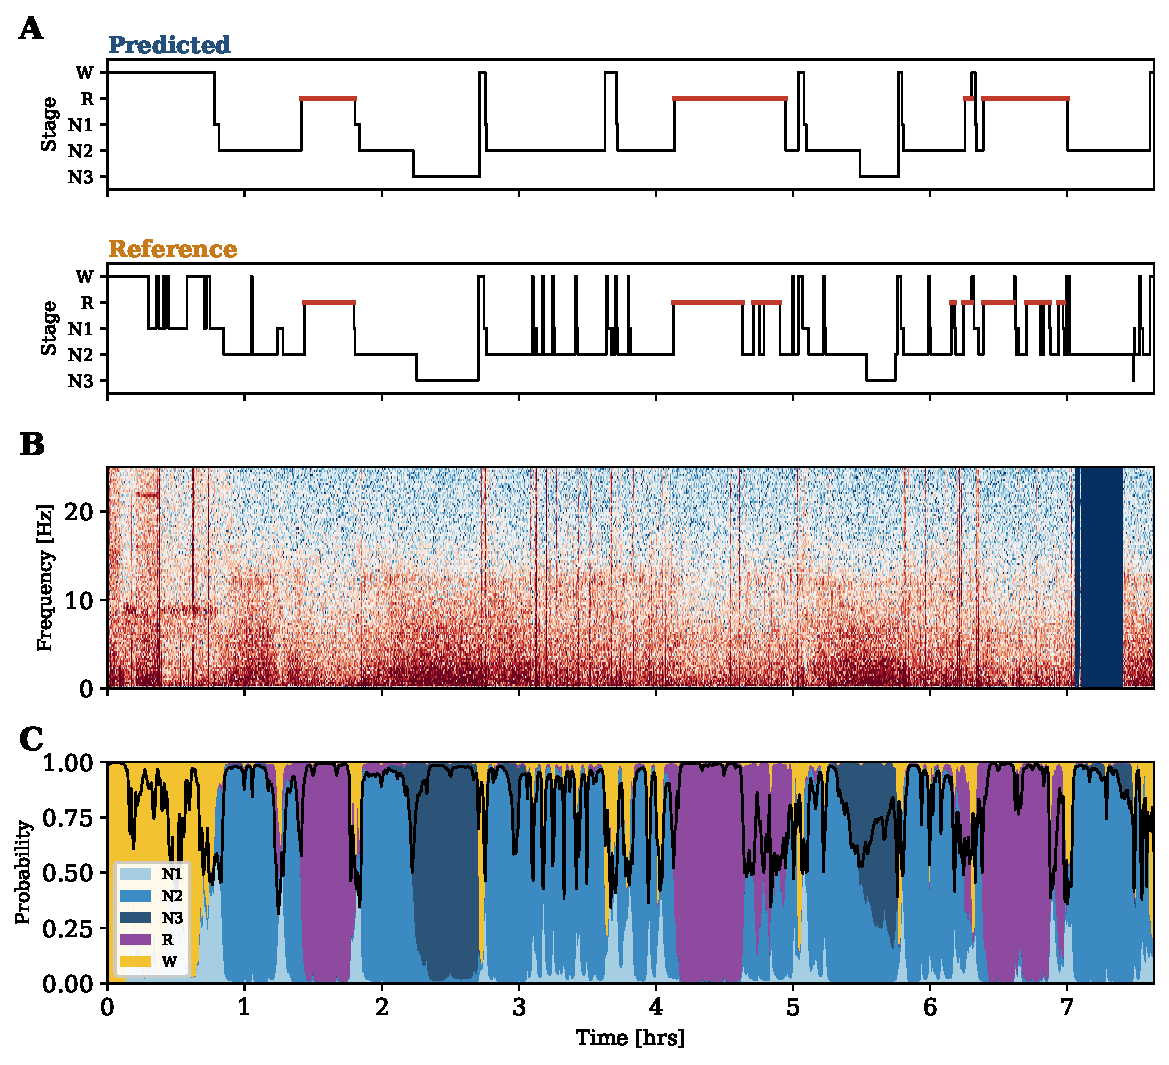
\includegraphics[width=0.86\textwidth]{figures/revision/fig_hypnogram_final.pdf}
\caption{An illustrative held-out night (patient SN90, three-seed MM-Net, staging accuracy
$0.83$). \textbf{(A)} Predicted and reference hypnograms, REM highlighted. \textbf{(B)} EEG
spectrogram, C4 derivation, $0$--$25$\,Hz. \textbf{(C)} Per-epoch stage-probability
ribbon; the black line is the maximum posterior.}
\label{fig:hypno}
\end{figure}

\subsection{Per-class Staging Performance}
Table~\ref{tab:perclass} breaks staging performance down by stage. MM-Net recovers Wake, N2 and REM at F1 $0.79$--$0.82$ and N3 at $0.72$; REM, whose ocular signature the sleep-adapted encoder receives, reaches $0.79$. N1, the transient stage between wake and
sleep, has the lowest F1 for every model on this cohort, and the raw multimodal CNN attains
the highest N1 F1, whereas MM-Net performs more strongly across the remaining stages. The row-normalised confusion matrix (Figure~\ref{fig:confusion}) shows the distribution of errors: N1 is absorbed mainly into Wake and N2, and part of N3 is read as N2. In the frozen-encoder
configuration, comparing the neural-only and full models shows little change in staging after
adding the cardiorespiratory stream: overall accuracy changes from $0.741$ to $\fzAcc$, N1 F1
increases by $0.019$ ($p=0.11$), and no per-stage difference reaches statistical significance
($p \geq 0.15$).

These results are consistent with the modality-ablation analysis in Section~\ref{sec:ablate}: staging depends primarily on the neural stream, whereas the cardiorespiratory stream supplies respiratory-event information and leaves staging performance essentially unchanged.

\begin{figure}[pos=H]
\centering
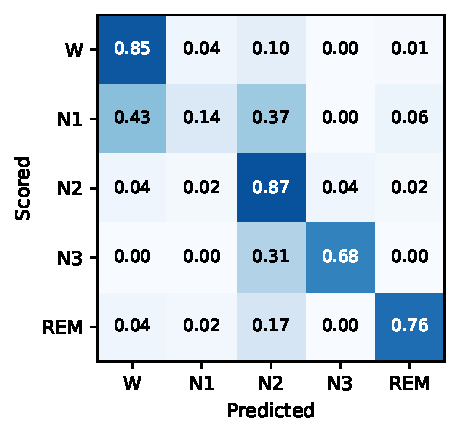
\includegraphics[width=0.55\textwidth]{figures/revision/fig_confusion_final.pdf}
\caption{Row-normalised confusion matrix for MM-Net (three-seed, pooled ten-fold test epochs,
hidden-Markov operating point). Errors concentrate on N1, which is absorbed into Wake and N2.}
\label{fig:confusion}
\end{figure}

\begin{table}[H]
\caption{Per-class staging F1 (Wake, N1, N2, N3, REM), ten-fold patient-independent, at the
hidden-Markov operating point (MM-Net: three-seed, pooled test epochs). Best per column in
\textbf{bold}.}
\label{tab:perclass}
\centering
\setlength{\tabcolsep}{6pt}
\begin{tabular}{lccccc}
\toprule
Model & W\,$\uparrow$ & N1\,$\uparrow$ & N2\,$\uparrow$ & N3\,$\uparrow$ & R\,$\uparrow$ \\
\midrule
Raw multimodal CNN & 0.74 & \textbf{0.37} & 0.73 & 0.56 & 0.67 \\
\textbf{MM-Net}    & \textbf{0.81} & 0.20 & \textbf{0.82} & \textbf{0.72} & \textbf{0.79} \\
\bottomrule
\end{tabular}
\end{table}

\subsection{Modality-Ablation Grid}
\label{sec:ablate}
This ablation is also our attribution method. Because the trainable network receives engineered descriptors and precomputed embeddings, and no raw spectrogram or EEG trace, a gradient heat-map or Grad-CAM would have no faithful spatial support on the neural side, which is where a staging attribution would be read; we therefore attribute each output by \emph{interventional} ablation, deleting a physiological channel and measuring the change. This is a falsifiable test of what each modality contributes.
The analysis uses the frozen-encoder configuration (Section~\ref{sec:results}), which stages
sleep at $\fzAcc$ accuracy ($\kappa$ $\fzK$) and detects respiratory events at $\fzAuc$ AUC
($\fzAp$ average precision). To test whether each modality carries the task to which its physiology is most closely related, we remove each modality in turn and keep the rest, on the same folds, with three seeds giving thirty fold-values per row (Table~\ref{tab:ablate}). The results show a task-specific separation between streams. Within the cardiorespiratory stream, the pattern differs from that obtained with the engineered features.

Removing the whole cardiorespiratory stream drops respiratory AUC from $\fzAuc$ to $0.654$, the largest effect in the ablation grid, and leaves staging untouched ($0.741$, n.s.).
Removing the neural stream does the reverse: staging falls from $\fzAcc$ to $0.680$ while
respiratory detection holds. No neural ablation significantly moves respiratory AUC and no
cardiorespiratory ablation significantly moves staging, so each stream serves the outcome its physiology is closest to.

Within the cardiorespiratory stream, however, only respiratory effort is individually necessary
($-0.038$ AUC, Holm $p=0.018$). Removing SpO$_2$, pulse/HRV, ECG or airflow individually costs at most $0.005$ AUC and none survives correction; SpO$_2$, the central input of the engineered-feature configuration, is among the least necessary channels here ($-0.002$, $p=1.00$). The five
individual removals sum to $-0.046$ AUC against $-0.128$ for removing the stream as a whole,
a factor of $2.8$. The learned encoder therefore distributes respiratory information redundantly across channels: each is individually dispensable because the others overlap with it, but the channels jointly are essential. That redundancy is clinically favourable, since
twelve of the ninety-nine recordings are missing at least one cardiorespiratory channel, and it is
physiologically coherent: the effort belts register the paradoxical thoraco-abdominal motion
of an obstructive event as it happens, whereas desaturation is a lagged consequence of it.

\subsection{What the Joint Objective Contributes}
\label{sec:joint}
As for the ablation grid, this comparison uses the frozen-encoder configuration. The ablation
grid establishes which physiology carries which output. It does not establish
whether the two outputs should share a network at all: a
model producing two outputs demonstrates integration, and integration alone does not
demonstrate benefit. The appropriate control is a pair of single-task models matched to the joint model in every other respect. The architecture, the ten folds, the three seeds, the optimiser, the budget and the cardiorespiratory bypass are those of the full model; only the surviving term of $\mathcal{L}=\mathcal{L}^{\mathrm{stg}}+\lambda\mathcal{L}^{\mathrm{apn}}$ differs, so the staging-only model still builds the cardiorespiratory stream and still feeds the respiratory head but never receives a respiratory gradient.

Joint training improves on training either task alone (Table~\ref{tab:joint}). Staging rises from $0.733$ to $\fzAcc$ accuracy, in nine folds of
ten (Wilcoxon on the ten fold-means, $p=0.014$), and $\kappa$ from $0.625$ to $\fzK$ on the
same nine. Respiratory AUC rises from $0.774$ to $\fzAuc$ in seven folds of ten ($p=0.049$).
Average precision moves $+0.005$ and does not separate ($p=0.63$), and is reported as a null result.

These gains support a narrow interpretation. The gains are small: $0.006$ accuracy against a fold-to-fold SD of $0.019$, and $0.007$ AUC against $0.038$, approximately one third and one fifth of the fold-to-fold variation. Their significance derives from consistency across folds, with nine and seven of ten folds moving in the same direction, which the paired test evaluates. The supported conclusion is that adding the respiratory task does not reduce staging performance and yields a small improvement, so the respiratory output is obtained without a loss of staging accuracy. We do not claim multi-task learning as a source of large gains here.

Two diagnostic cells verify the comparison. The respiratory-only
model stages at $0.303$ accuracy and $\kappa$ $0.039$, and the staging-only model detects at
$0.495$ AUC. Both are at chance for their untrained head, which confirms that the switch isolated the loss and that the other objective was inactive.

\begin{table}[H]
\caption{Joint multi-task training compared with matched single-task models using the same architecture, folds, seeds, and training budget (frozen-encoder configuration). The lower rows report the untrained head as a control for loss isolation.}
\label{tab:joint}
\centering
\small
\setlength{\tabcolsep}{5pt}
\begin{tabular}{llccc}
\toprule
Trained on & Metric & Single & Joint & $p$ \\
\midrule
\multirow{2}{*}{Staging only}
 & Accuracy & $0.733$ & $\mathbf{\fzAcc}$ & $\mathbf{0.014}$ \\
 & $\kappa$ & $0.625$ & $\mathbf{\fzK}$   & $\mathbf{0.014}$ \\
\addlinespace[2pt]
\multirow{2}{*}{Respiratory only}
 & AUC & $0.774$ & $\mathbf{\fzAuc}$ & $\mathbf{0.049}$ \\
 & AP  & $0.414$ & $0.419$           & $0.63$ \\
\midrule
\multicolumn{5}{@{}l}{\emph{Untrained heads, reported as the check that the switch worked}}\\[1pt]
Respiratory only & Accuracy & $0.303$ & --- & --- \\
Staging only     & AUC      & $0.495$ & --- & --- \\
\bottomrule
\end{tabular}
\end{table}

\subsection{Recordings With an Incomplete Montage}
In the frozen-encoder configuration, those twelve recordings are scored with the absent channels zero-filled instead of being excluded, which raises the question of whether the network relies on missingness patterns instead of physiology. The evidence indicates that it does not. Removing all twelve from the pooled respiratory evaluation moves AUC from $0.777$ to $0.775$ and moves average precision the other way, from $0.419$ to $0.439$, so the respiratory result does not depend on these recordings. Predicted per-patient burden is independent of whether a montage was complete ($p=0.91$), so missingness provides no usable shortcut.

Staging is lower on those twelve, $0.670$ against $0.743$ ($p=0.017$), which requires a control comparison. The neural-only configuration receives no
cardiorespiratory channel at all and so has nothing zero-filled, yet it shows the same
gap in the same direction, $0.689$ against $0.744$ ($p=0.040$). Most of the difference is therefore attributable to the recordings themselves, which are also harder for a model that does not receive the missing channels. On those twelve the
full model sits $0.019$ below neural-only, which at $n=12$ is not distinguishable from
noise (Wilcoxon $p=0.18$), so a small cost can be bounded but not excluded. On the
eighty-seven complete recordings the two agree to within $0.002$.

A zero-filled channel can resemble a flat channel after per-patient standardisation, so we
also retrained two variants with explicit missing-input information on the same folds using
seed $42$. The first appends seven per-recording channel-availability flags to the pooled
cardiorespiratory representation. The second combines these flags with channel dropout,
removing each available channel and its flag during training with probability $0.15$. Under
the same seed, the reference configuration reaches $0.734$ accuracy and $0.779$ respiratory
AUC, with AUCs of $0.779$ on the $87$ complete recordings and $0.791$ on the $12$ incomplete
recordings. Availability flags yield $0.739$ accuracy and $0.782$ pooled AUC, with subgroup
AUCs of $0.776$ and $0.835$; flags with channel dropout yield $0.738$, $0.779$, $0.770$, and
$0.826$, respectively. Pooled performance is therefore essentially unchanged. Both explicit
missingness treatments increase AUC on the incomplete-recording subgroup by about $0.04$;
with twelve patients and one seed, this subgroup difference is treated as suggestive.
In this configuration, attention-based and concatenation fusion yield similar staging and detection performance (Section~\ref{sec:method}), so the fusion mechanism has little effect on these results.

\begin{table}[H]
\caption{Modality-ablation grid (leave-one-out, frozen-encoder configuration), ten-fold
patient-independent, three seeds. Each row removes one modality and keeps the rest; cells are means over
thirty fold-values. $p$ is Wilcoxon on the ten fold-means, Holm-corrected across the
nine ablations within each metric and \textbf{bold} where it clears $0.05$; the
floor at this sample size is $0.018$.}
\label{tab:ablate}
\centering
\setlength{\tabcolsep}{14pt}
\begin{tabular}{lcccc}
\toprule
Modality removed & Staging acc\,$\uparrow$ & Holm $p$ & Respiratory AUC\,$\uparrow$ & Holm $p$ \\
\midrule
 none (full model)        & $0.739 \pm 0.020$   & ---                 & $0.782 \pm 0.038$   & --- \\
 EEG (neural)             & $0.680$             & $\mathbf{0.018}$    & $0.774$             & $0.92$ \\
 EOG (ocular)             & $0.731$             & $0.08$              & $0.777$             & $1.00$ \\
 EMG (muscle)             & $0.735$             & $1.00$              & $0.778$             & $1.00$ \\
 SpO$_2$                  & $0.742$             & $1.00$              & $0.780$             & $1.00$ \\
 respiratory effort       & $0.741$             & $1.00$              & $0.744$             & $\mathbf{0.018}$ \\
 pulse / HRV              & $0.741$             & $1.00$              & $0.785$             & $1.00$ \\
 ECG                      & $0.737$             & $1.00$              & $0.777$             & $1.00$ \\
 airflow                  & $0.740$             & $1.00$              & $0.778$             & $1.00$ \\
 all cardiorespiratory    & $0.741$             & $1.00$              & $0.654$             & $\mathbf{0.018}$ \\
\bottomrule
\end{tabular}
\end{table}

\subsection{Physiological Validity of the Respiratory Read-out}
\label{sec:noflow}
Because the events were scored from airflow, predominant reliance on that channel could
produce a circular association. In the frozen-encoder configuration, removing the airflow features leaves detection essentially unchanged, at $\noflowAuc$ AUC (Table~\ref{tab:ablate}), within one fold standard deviation of the full $\fzAuc$. After retraining, the remaining scoring-relevant channels recover nearly
all respiratory discrimination. Respiratory effort provides the strongest individual contribution;
the smaller effects of the other single-channel removals indicate that the
learned encoder represents them redundantly. This indicates that detection is supported by
physiological correlates of disordered breathing. This pattern is consistent with physiology: the effort belts register the paradoxical thoraco-abdominal motion of an obstructive event while it is happening, whereas desaturation follows it by several breaths.

\subsection{Respiratory Baselines and Per-event-type Detection}
The respiratory task is compared with established detectors on the same folds and the same
epoch labels (Table~\ref{tab:resp}). The classical baselines read the $14$ engineered
cardiorespiratory descriptors; MM-Net reads the raw signal through its learned encoder (in the
frozen-encoder configuration its own score on the $14$ descriptors is $0.698$,
Table~\ref{tab:repr}). A clinical desaturation rule reaches $0.595$ AUC, logistic regression
$0.603$, and gradient boosting $0.673$; a random classifier scores $0.160$ average precision, the
event prevalence. MM-Net reaches $\mmAuc$ AUC and $\mmAp$ average precision, $0.152$ AUC and
$0.197$ average precision above gradient boosting. Detection also separates by event type: the
model scores $0.810$ AUC on hypopneas (the mild, dominant $82\%$ of event epochs), $0.898$ on
obstructive apneas, and $0.946$ on central apneas. It is strongest on the most severe events, and the pooled AUC is dominated by the more numerous hypopneas.

To compare the proposed representation against end-to-end waveform detectors, we added two
raw-signal respiratory baselines. Each uses a per-epoch convolutional encoder over the
$25$\,Hz waveform followed by a bidirectional LSTM across $20$-epoch windows and is trained
with the same epoch labels, folds, early-stopping rule, and positive-class weighting
($n_-/n_+$). The first reads summed respiratory effort alone, matching the input configuration
of Nassi~\emph{et al.}~\cite{nassi2022effortbelt}; the second reads all seven raw
cardiorespiratory channels. With a single seed, the effort-only model reaches
$0.602 \pm 0.057$ AUC and $0.252$ average precision, while the seven-channel model
reaches $0.733 \pm 0.036$ AUC and $0.366$ average precision (Table~\ref{tab:resp}).
MM-Net reaches $\mmAuc$ AUC and $\mmAp$ average precision using these channels and nasal
pressure together with the neural stream and shared temporal context.

Figure~\ref{fig:rocpr} shows the operating characteristics behind these numbers, computed
from the pooled held-out predictions of all ten folds. The precision--recall panel is the more informative of the two: respiratory events occupy $16\%$ of epochs, and under this class imbalance a ROC curve can overstate detector performance. Read at fixed sensitivity, the trade-off is
explicit: at $0.80$ sensitivity MM-Net holds $0.70$ specificity, and at $0.90$ sensitivity
$0.53$. Pooling every fold's epochs into a single curve is not the same estimator as averaging
the ten per-fold scores: pooling weights folds by epoch count and mixes their score scales,
giving a pooled AUC of $0.828$ against the cross-validated $\mmAuc \pm 0.035$ reported in
Table~\ref{tab:resp}; at $0.003$ the difference is a tenth of one fold standard deviation.

\begin{figure}[pos=H]
\centering
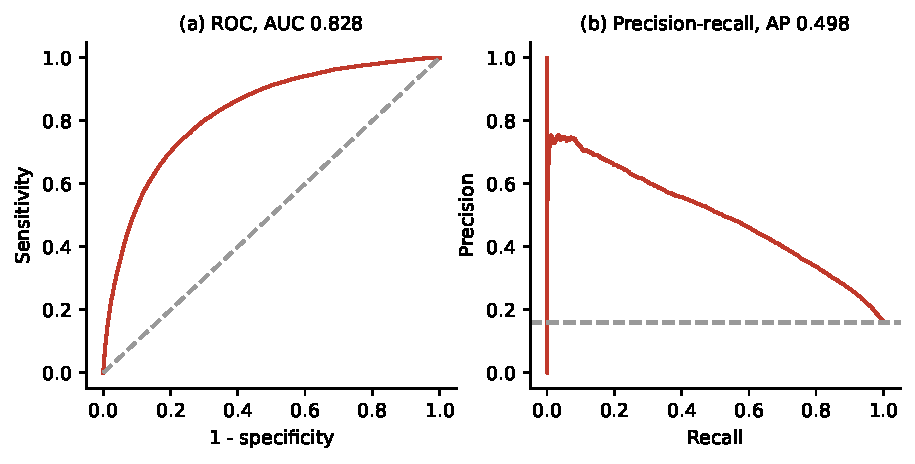
\includegraphics[width=0.8\textwidth]{figures/revision/fig_roc_pr_final.pdf}
\caption{Respiratory-event detection by MM-Net (three-seed), pooled over the ten
patient-independent test folds. \textbf{(a)} ROC curve. \textbf{(b)} Precision--recall; the
dashed line is the $0.160$ event prevalence, the no-skill floor.}
\label{fig:rocpr}
\end{figure}

\begin{table}[H]
\caption{Respiratory-event detection on iSLEEPS. (A) Comparison with classical and raw-signal baselines on the same folds and (B) MM-Net AUC by respiratory-event type. Bold denotes the best value in each comparison.}
\label{tab:resp}
\centering
\small
\begin{tabular}{lcc}
\toprule
\multicolumn{3}{l}{\textit{(a) Detection method}}\\
\midrule
Method & AUC\,$\uparrow$ & AP\,$\uparrow$ \\
\midrule
Desaturation rule    & 0.595 & 0.207 \\
Logistic regression  & 0.603 & 0.211 \\
Gradient boosting    & 0.673 & 0.290 \\
Raw effort belt$^{\S}$~\cite{nassi2022effortbelt} & 0.602 & 0.252 \\
Raw seven channels$^{\S}$ & 0.733 & 0.366 \\
MM-Net, single model & 0.815 & 0.471 \\
\textbf{MM-Net, three-seed} & \textbf{0.825} & \textbf{0.487} \\
\bottomrule
\end{tabular}

\vspace{4pt}
\begin{tabular}{lcc}
\toprule
\multicolumn{3}{l}{\textit{(b) MM-Net AUC by event type}}\\
\midrule
Event type & Positive epochs & AUC\,$\uparrow$ \\
\midrule
Hypopnea    & 11{,}921 & 0.810 \\
Obstructive & 1{,}722  & 0.898 \\
Central     & 832      & \textbf{0.946} \\
\bottomrule
\end{tabular}
\end{table}

\subsection{AHI Estimation and Clinical Severity}
\label{sec:ahi}
MM-Net's AHI estimate (Section~\ref{sec:ahimethod}) tracks the annotated index across the full
severity range: Spearman $\rho=\mmRho$ over the $99$ test patients, a mean absolute error of
$10.4$ events/h, and $54\%$ of patients placed in the correct AASM severity band (weighted
$\kappa$ $0.45$; Table~\ref{tab:ahi}, Figure~\ref{fig:ahi}). Two references place this result.
The clinical AHI recorded with the corpus agrees with the annotated index at $\rho=0.687$, so
MM-Net's estimate is closer to the annotations than the clinical index itself; against that
clinical index MM-Net reaches $\rho=0.633$. In the expected-count formulation, summing the onset scores over decoded sleep counts closely spaced events separately, whereas thresholding the scores into runs would merge them, and normalising by decoded sleep time matches the denominator of the clinical index.

We also trained a dedicated event detector, a one-dimensional U-Net with a recurrent
bottleneck operating at one-second resolution on the raw cardiorespiratory signals, with its
counting rule chosen on validation patients. On its own it reaches $\rho=0.669$; averaged with MM-Net it lowers the error to $9.7$ events/h and raises severity agreement to $55\%$ (weighted $\kappa$ $0.51$), and MM-Net alone yields the highest correlation. The AHI is therefore
available from the staging model itself, without a separate detector.

Staging remains stable across sleep-disordered-breathing severity: accuracy is $0.784$ in
patients with a normal clinical AHI, $0.754$, $0.764$ and $0.758$ in the mild, moderate and
severe groups, with no significant ordered trend (Jonckheere--Terpstra $p=0.20$;
Table~\ref{tab:severity}). The model therefore stages the most severely affected patients nearly as well as those without sleep-disordered breathing, the group in which both outputs are most clinically relevant.

\begin{table}[H]
\caption{AHI estimation on iSLEEPS ($99$ test patients, stages decoded by MM-Net). Severity:
AASM bands; $\kappa_w$ linearly weighted. Last column: Spearman $\rho$ against the clinical AHI
recorded with the corpus. The last row gives the agreement of the clinical AHI with the
annotated AHI.}
\label{tab:ahi}
\centering
\small
\setlength{\tabcolsep}{3pt}
\adjustbox{max width=\textwidth}{%
\begin{tabular}{@{}lccccc@{}}
\toprule
Estimator & $\rho$\,$\uparrow$ & MAE\,$\downarrow$ & Sev.\ acc\,$\uparrow$ & $\kappa_w$\,$\uparrow$ & $\rho_{\mathrm{clin}}$\,$\uparrow$ \\
\midrule
Event detector & 0.669 & 11.7 & 0.45 & 0.44 & 0.569 \\
\textbf{MM-Net} & \textbf{0.765} & 10.4 & 0.54 & 0.45 & \textbf{0.633} \\
MM-Net $+$ event detector & 0.742 & \textbf{9.7} & \textbf{0.55} & \textbf{0.51} & 0.625 \\
\midrule
Clinical vs.\ annotated AHI & 0.687 & & & & \\
\bottomrule
\end{tabular}}
\end{table}

\begin{figure}[pos=H]
\centering
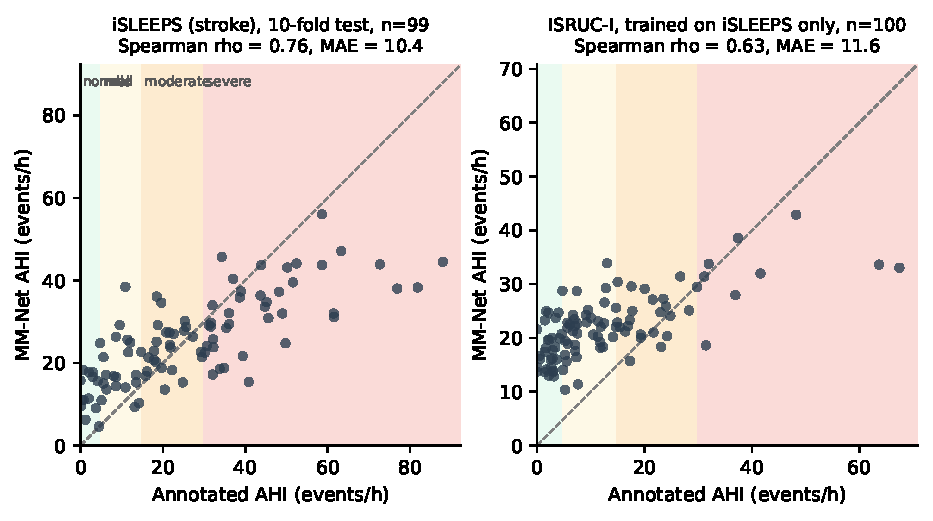
\includegraphics[width=0.72\textwidth]{figures/revision/fig_rev_ahi.pdf}
\caption{MM-Net AHI estimate against the annotated AHI. Left: iSLEEPS, ten-fold test patients.
Right: ISRUC-I, MM-Net trained on iSLEEPS only and applied without retraining
(Section~\ref{sec:external}). Shading marks the AASM severity bands; the dashed line is
identity.}
\label{fig:ahi}
\end{figure}

\begin{table}[H]
\caption{Sleep-staging accuracy of MM-Net across AASM severity groups of the clinical AHI in
iSLEEPS. Values are mean $\pm$ SD across patients; the ordered-group trend is not significant
(Jonckheere--Terpstra $p=0.20$).}
\label{tab:severity}
\centering
\small
\begin{tabular}{lccc}
\toprule
AHI band & AHI (events/h) & Patients & Staging acc\,$\uparrow$ \\
\midrule
Normal   & $<5$       & 15 & $0.784 \pm 0.057$ \\
Mild     & $5$--$15$  & 23 & $0.754 \pm 0.092$ \\
Moderate & $15$--$30$ & 23 & $0.764 \pm 0.083$ \\
Severe   & $\geq 30$  & 38 & $0.758 \pm 0.078$ \\
\bottomrule
\end{tabular}
\end{table}

\subsection{Permutation Importance: a Second, Independent Attribution}
The ablation grid establishes what the model \emph{needs}: remove a modality, retrain, and observe which output degrades. A complementary question is what a \emph{trained} model actually
uses. We therefore permute each modality's features across epochs at inference time in the
frozen-encoder configuration, so the
channel is still present but no longer aligned to the epoch it describes, and measure the
drop, averaged over three shuffles and the ten fold models.

The two methods can disagree, because a model may need a channel during training yet weight it
lightly afterwards. On staging they do not: permuting the neural features costs $0.284$ staging
accuracy against $0.030$ for the ocular and $0.006$ for the muscle channel, the same ordering
the ablation gives, and the rank correlation between the two attributions is $\rho=0.833$
($p=0.010$).

On the respiratory head the agreement is narrower, and we report the two attributions
separately. Both methods place respiratory effort first by a wide margin: $0.038$ AUC under retraining, $0.071$ under permutation, in each case substantially above the second-ranked channel. The remaining four cardiorespiratory channels, however, have retraining effects that are not distinguishable from zero, so their rank order is not informative and the correlation over the five is correspondingly uninformative ($\rho=0.381$, $p=0.35$).

Permutation effects are largest for respiratory effort ($0.071$ AUC), airflow ($0.027$), and SpO$_2$ ($0.016$), followed by pulse/HRV ($0.012$), with the remaining channels below $0.006$. The magnitude ordering therefore identifies respiratory effort as the dominant input used by the fitted respiratory model. Retraining and permutation measure complementary properties. Retraining after channel removal measures whether the remaining inputs can compensate for the missing signal, whereas permutation measures reliance of the fitted model on the aligned input. SpO$_2$, for example, produces a $0.002$ AUC change after retraining without it but a $0.016$ decrease when shuffled at inference. Both analyses identify respiratory effort as the strongest individual
cardiorespiratory contributor.

\subsection{Healthy-Trained Models Applied to the Injured Brain}
\label{sec:domaingap}
To examine cross-dataset transfer without adaptation, we trained three staging
architectures on Sleep-EDF: a four-channel CNN, a CNN with a BiLSTM over epochs,
and StagingSeqNet. Their Sleep-EDF accuracies range from $0.806$ to $0.855$ with
$\kappa=0.73$--$0.81$. Applied zero-shot to the 99 iSLEEPS patients, the same
checkpoints reach $0.306$--$0.312$ accuracy with $\kappa=0.09$--$0.13$.
Predictions shift strongly toward Wake, which accounts for $62$--$79\%$ of
predicted epochs, while N2 accounts for only $1$--$5\%$ despite representing
$42.3\%$ of the iSLEEPS epochs.

A held-out Sleep-EDF implementation check using the same preprocessing reaches
$0.8682$ accuracy ($0.8667 \pm 0.0415$ per recording), confirming that the
healthy-sleep performance is retained through the evaluation pipeline. The
zero-shot result must nevertheless be interpreted under both population and
montage shift: Sleep-EDF uses Fpz-Cz and Pz-Oz, whereas iSLEEPS uses C4 and O2.
The transfer experiment therefore establishes a substantial dataset shift but
does not isolate stroke as its sole source.

MM-Net reaches $0.864 \pm 0.030$ accuracy with $\kappa=0.810$ under
subject-independent evaluation on Sleep-EDF, compared with $\mmAcc$ on iSLEEPS. Across the retrained staging baselines, the corresponding
healthy-to-iSLEEPS decreases range from approximately $0.12$ to $0.15$.
These cross-system differences are descriptive because channel configurations
and representations differ across models, but they consistently show that
staging performance depends strongly on the target dataset and population.

Sleep-EDF folds are split at the subject level because individual participants
contribute two recording nights, preventing recordings from the same subject
from appearing in both training and test folds.



\subsection{Stream Representations}
\label{sec:repr}
The representation experiments use the frozen-encoder configuration: engineered features together with a frozen self-supervised embedding for the neural stream and a learned convolutional encoder over the raw cardiorespiratory signal. Both representation choices were evaluated experimentally before selection. Each family below holds every other hyperparameter fixed and varies one factor, over the same three seeds and ten patient-independent folds, with Holm correction within the family and every test on the ten fold-means.

The cardiorespiratory experiments show progressively higher respiratory discrimination as the representation is enriched. Each block of Table~\ref{tab:repr} holds the other stream at its baseline, so no single
row there is the full model, and the two baselines differ: the cardiorespiratory block runs
the $188$ neural descriptors without the pretrained embedding, while the neural block runs the
$14$ engineered cardiorespiratory descriptors. Consequently, the two blocks report different respiratory AUC for what both call an engineered-feature reference ($0.698$ against $0.685$), and the adopted cardiorespiratory row reads $0.740$ staging accuracy against the headline $\fzAcc$, which adds the pretrained embedding on top of it. The upper block replaces the $14$ engineered cardiorespiratory features
with progressively richer representations of the same underlying signal. Every step is
significant, and the ordering identifies where the limitation lies. A \emph{random} nonlinear expansion of the same $14$ numbers recovers $0.018$ AUC, a gain obtained without additional input information and from added capacity alone, indicating that the summary features leave nonlinear structure unrepresented. A random linear projection of the raw waveform adds a further $0.016$, so part of what the features discard is recoverable without learned parameters. The learned
convolutional encoder reaches $0.782$, $0.084$ above the engineered features.

These results indicate that respiratory performance is primarily constrained by the representation of the cardiorespiratory stream; the downstream detector is held fixed throughout the comparison.

The same representation search also evaluated MOMENT~\cite{goswami2024moment} as a frozen
time-series encoder for the cardiorespiratory stream. Pretrained weights yield a respiratory
AUC of $0.808$, while randomly initialised frozen weights yield $0.795$, with comparable
staging accuracy in both cases (Table~\ref{tab:repr}). The randomly initialised variant is also
the time-series encoder selected most often by the nested procedure in
Section~\ref{sec:nested}. These controls support the representation-level finding across
alternative high-capacity encoders. The learned convolutional encoder is retained in MM-Net as
the compact implementation: it contains $0.155$ million trainable parameters, is trained end
to end with the rest of the network, and introduces no external model dependency, compared
with the $341$ million frozen parameters of MOMENT.

On the neural side, a frozen pretrained encoder complements the expert features without replacing them. The lower block of Table~\ref{tab:repr} varies the neural representation with the
cardiorespiratory stream held at the engineered features. Used alone, the frozen encoder is
significantly \emph{worse} than the $188$ features ($-0.029$, Holm $p=0.008$): pretraining on
healthy scalp EEG does not by itself substitute for physiology chosen for this task.
Concatenated with the features it adds $+0.008$ accuracy (Holm $p=0.006$), and a second
pretrained encoder on top of the first adds nothing further ($-0.004$, $p=0.56$).

These results support a narrow interpretation: expert physiology and self-supervised pretraining encode partly different information, so their combination outperforms either alone; the complementarity, however, saturates after one pretrained encoder, which does not support stacking several foundation models.

\begin{table}[H]
\caption{Comparison of cardiorespiratory and neural representations (frozen-encoder configuration). Each block varies one representation while holding the other stream fixed; values are mean $\pm$ SD across thirty fold-seed runs, with Holm-corrected comparisons against the engineered-feature baseline. $^{\dagger}$ denotes MOMENT-1-large.}
\label{tab:repr}
\centering
\begin{tabular*}{\textwidth}{@{\extracolsep{\fill}} l l c c c c @{}}
\toprule
Representation & Variant & Resp.\ AUC\,$\uparrow$ & Staging acc\,$\uparrow$ & $\Delta$ & Holm $p$ \\
\midrule
\multirow{6}{*}{\emph{Cardiorespiratory}}
 & $14$ engineered features               & $0.698 \pm 0.051$ & $0.736 \pm 0.014$ & ---      & ---      \\
 & random nonlinear expansion of the $14$ & $0.715 \pm 0.047$ & $0.737 \pm 0.018$ & $+0.018$ & $0.012$   \\
 & random linear projection of raw signal & $0.731 \pm 0.044$ & $0.735 \pm 0.021$ & $+0.034$ & $0.012$   \\
 & learned CNN, $0.155$\,M (adopted)      & $0.782 \pm 0.040$ & $0.740 \pm 0.019$ & $+0.084$ & $\mathbf{0.010}$ \\
 & random-init.\ time-series encoder$^{\dagger}$ & $0.795 \pm 0.045$ & $0.737 \pm 0.017$ & $+0.097$ & $0.010$ \\
 & pretrained time-series encoder$^{\dagger}$    & $\mathbf{0.808 \pm 0.042}$ & $0.734 \pm 0.018$ & $+0.110$ & $0.010$ \\
\midrule
\multirow{4}{*}{\emph{Neural}}
 & $188$ engineered features            & $0.685 \pm 0.041$ & $0.741 \pm 0.016$ & ---      & ---      \\
 & frozen pretrained encoder alone      & $0.681 \pm 0.033$ & $0.712 \pm 0.033$ & $-0.029$ & $0.008$   \\
 & features $+$ pretrained (adopted)    & $0.690 \pm 0.037$ & $\mathbf{0.749 \pm 0.018}$ & $+0.008$ & $\mathbf{0.006}$ \\
 & features $+$ two pretrained encoders & $0.684 \pm 0.043$ & $0.745 \pm 0.018$ & $+0.004$ & $0.23$   \\
\bottomrule
\end{tabular*}
\end{table}

\subsection{Integrating the Sleep-Adapted Encoder}
\label{sec:integration}
Table~\ref{tab:components} builds MM-Net from the frozen-encoder configuration one change at a
time, every row on the same folds and seeds. Uniform class weights and cross-attention fusion
contribute $+0.009$ together. The largest change comes from the encoder. A sleep-adapted encoder whose
training embeddings are cross-fitted but not aligned moves the three-seed accuracy by only
$+0.002$ ($p=0.63$) and falls below the frozen encoder in five folds of ten, by up to $0.023$ in
the fold where the cross-fitted and full encoders agree least (embedding cosine similarity
$0.53$). Aligning the embedding spaces turns the same encoder into a gain of $+0.014$
($0.755\rightarrow0.769$, $p=0.020$), and of $+0.015$ for the single model in nine folds of ten
($p=0.027$). The complete MM-Net adds three elements that serve REM and the respiratory head more than overall staging: the ocular channels in the encoder, which raise the encoder's own accuracy from $0.709$ to $0.732$, nasal pressure, and the epoch alignment of Section~\ref{sec:data}. With all three, staging is $\mmAcc$; an EEG-only encoder in the same model
gives $0.765$, which is indistinguishable ($p=0.38$), and MM-Net uses the EEG and EOG encoder in
every cohort of this study.

On its own, the sleep-adapted encoder reaches $0.732$ on single epochs without a temporal model, against $0.647$ for the frozen encoder read by logistic regression.
The remaining components of MM-Net add to this performance. With the engineered descriptors, the
cardiorespiratory stream and the temporal decoder, the same encoder yields $\mmAccS$ as a single
model, $+0.024$ in eight folds of ten ($p=0.014$); on ISRUC-I the corresponding gain is $+0.012$
($p=0.014$; Section~\ref{sec:external}). Figure~\ref{fig:tsne} shows what adaptation changes in
the representation: held-out epochs that the frozen encoder spreads across one mixed cloud
form stage-specific clusters after adaptation, with Wake, REM and N3 separated (silhouette by
stage $-0.045\rightarrow0.047$).

\begin{table}[H]
\caption{From the frozen-encoder configuration to MM-Net on iSLEEPS, one change per row (upper
block), and the complete model (lower block); same ten folds and three seeds throughout. $p$:
Wilcoxon on fold means against the row marked ref.}
\label{tab:components}
\centering
\small
\setlength{\tabcolsep}{3pt}
\adjustbox{max width=\textwidth}{%
\begin{tabular}{@{}lccc@{}}
\toprule
Configuration & Single & 3-seed & $p$ \\
\midrule
Frozen encoder, class weights, concatenation & 0.738 & 0.749 & \\
\ \ $+$ uniform class weights & 0.744 & 0.754 & \\
\ \ $+$ cross-attention fusion & 0.747 & 0.755 & ref. \\
\ \ $+$ sleep-adapted encoder, cross-fitted, not aligned & 0.752 & 0.757 & 0.63 \\
\ \ $+$ ridge alignment (7 channels) & \textbf{0.762} & \textbf{0.769} & \textbf{0.020} \\
\midrule
MM-Net: EEG$+$EOG encoder, 8 channels, epoch-aligned & 0.756 & 0.763 & \\
\ \ with an EEG-only encoder & 0.757 & 0.765 & \\
\bottomrule
\end{tabular}}
\end{table}

\begin{figure}[pos=H]
\centering
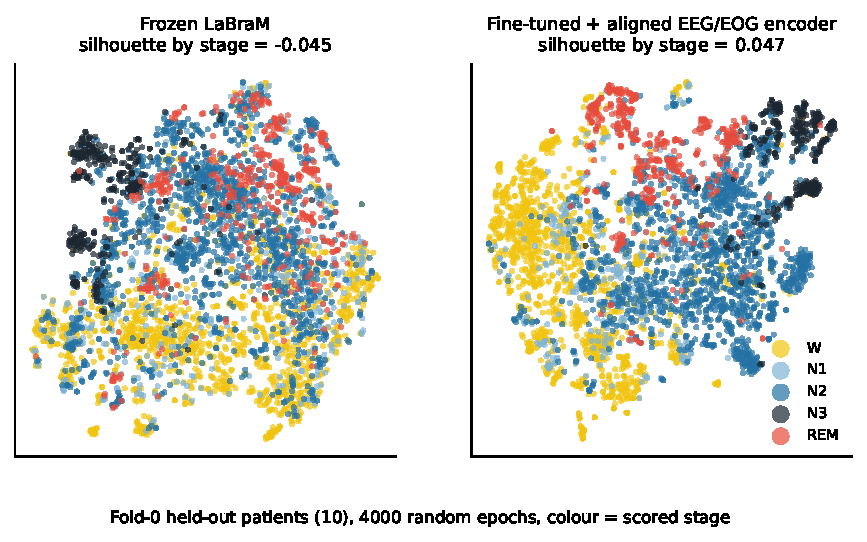
\includegraphics[width=0.72\textwidth]{figures/revision/fig_rev_tsne.pdf}
\caption{t-SNE~\cite{vandermaaten2008tsne} of $4000$ epochs from the ten held-out patients of
one fold, coloured by scored stage. Left: frozen LaBraM. Right: the sleep-adapted, aligned
EEG/EOG encoder used in MM-Net.}
\label{fig:tsne}
\end{figure}

\subsection{The Two Loss Constants}
\label{sec:losssens}
Two constants in Section~\ref{sec:method} were fixed by argument:
the task balance $\lambda=1$ and the positive weight $\pi=n_-/n_+$, which is $5.35$ on this
corpus. Equal coefficients do not imply equal influence, because the two terms differ in scale and curvature; $\lambda=1$ is therefore a nominal choice. We therefore swept each in the frozen-encoder configuration with everything else at its reference setting, three seeds by ten folds per value, and evaluate both heads at every point, because the relevant outcome is the trade-off between the heads.

No trade-off is observed, and the effect of either constant is small. Across $\lambda$ from
$0.25$ to $4$
staging accuracy spans $0.003$ and respiratory AUC $0.018$, and across $\pi$ from $1$ to $11$
they span $0.003$ and $0.007$; the fold-to-fold standard deviations are $0.019$ and $0.038$.
Both heads attain their maximum at the same $\lambda$, which is inconsistent with a
compromise setting: were $\lambda=1$ balancing one task against the other, the two curves
would peak on opposite sides of it.

Neither reference value is the maximum of those tested. Staging is highest at $\lambda=2$
($0.7403$) and at $\pi=11$ ($0.7422$), and respiratory AUC at $\lambda=2$ ($0.7840$) and
$\pi=8$ ($0.7846$). All of these margins are below a fifth of a fold standard deviation, so
the sweep does not identify better settings; it establishes that the objective is insensitive
to both constants across the range examined, and that fixing them a priori has no measurable
cost on this corpus.

\subsection{Calibration and Selective Prediction}
Clinical use requires information on both the accuracy of the model and the reliability of its confidence. Two measurements address this for the frozen-encoder configuration, both computed on held-out epochs with the raw posteriors before HMM smoothing.

% The model is \emph{overconfident}: expected calibration error, over ten equal-width confidence
% bins weighted by occupancy and ignoring bins holding fewer than fifty epochs, is $0.076$, and
% the gap runs one way in every bin: epochs it scores above $0.9$ are correct $88\%$ of the time.
% Stated confidences should therefore be read as ordered, not as probabilities, which is the
% displacement Section~\ref{sec:method} derives arriving in the measurement.

The model shows some overconfidence. Its expected calibration error is $0.076$. We calculate this value using ten equal-width confidence bins weighted by occupancy. Bins containing fewer than fifty epochs are excluded from the calculation. The same calibration pattern appears across the confidence bins. For example, epochs with confidence scores above $0.9$ are correct $88\%$ of the time. The confidence scores are therefore most useful for ordering predictions by certainty. Section~\ref{sec:method} explains why their numerical values differ from calibrated probabilities.




Abstention requires only a correct ranking of confidence. Applying split-conformal prediction with the
fold's validation patients as the calibration set gives empirical coverage that tracks the
target closely ($0.894$ at a $0.90$ target, $0.943$ at $0.95$). At $\alpha=0.10$ the model
returns a single stage for $45.8\%$ of epochs and is correct on $86.9\%$ of those, against
$59.1\%$ on the epochs where it returns a larger set. Abstention therefore selects the more difficult epochs and concentrates on the stage that is hardest for human scorers: N1 receives a singleton set only $19\%$ of the time, the lowest of any stage and the stage on which human scorers agree least.

The coverage estimates are subject to two limitations that do not directly affect the observed abstention behavior. The
calibration patients are the same patients that stopped training, so their labels have already
influenced which checkpoint was kept and they are not the independent calibration sample
split-conformal theory assumes; the coverage we report is therefore empirical and carries no
guarantee. In addition, epochs within a night are strongly dependent, so the exchangeable unit is closer to the patient than to the epoch; the reported values are therefore marginal rates across pooled epochs and do not represent coverage for a new patient or within any one stage. A calibration split disjoint from early stopping would resolve both issues; such a split was not used here.

\subsection{External Validation on Independent Cohorts}
\label{sec:external}
Ten-fold cross-validation is patient-independent but remains within one corpus, one centre
and one acquisition protocol. MM-Net is therefore evaluated in two further settings: trained
and tested on independent cohorts under subject-independent cross-validation, with the encoder
adapted, cross-fitted and aligned inside each fold exactly as on iSLEEPS; and trained on all
$99$ iSLEEPS patients and applied unchanged to external cohorts, with no re-fitted parameter,
threshold or transition matrix (per-recording standardisation is applied, as in training).

\paragraph{Trained and tested on ISRUC-Sleep} ISRUC-I is evaluated with ten
subject-independent folds of $80$ training, $10$ validation and $10$ test subjects, and
ISRUC-II and III together with six folds that keep both nights of a subject on the same side.
On ISRUC-I MM-Net reaches $0.803$ accuracy, macro-F1 $0.765$ and $\kappa$ $0.744$
(Table~\ref{tab:isruccv}). It is ahead of the frozen-encoder configuration in nine folds of ten
($+0.018$, $p=0.004$), and the gain extends to respiratory detection
($0.872\rightarrow0.889$ AUC) and to the AHI ($\rho$ $0.523\rightarrow0.590$, mean absolute error
$6.6$ events/h). As on iSLEEPS, MM-Net is ahead of its sleep-adapted encoder used alone ($0.792$;
$+0.012$ in eight folds of ten, $p=0.014$). The reimplemented baselines, retrained on MM-Net's
ISRUC-I folds with three seeds, reach $0.691$ to $0.778$; MM-Net is ahead of each of them in nine
or ten folds of ten, by $+0.025$ over the corpus LSTM to $+0.112$ over Huttunen~et~al. (Holm
$p=0.018$, the minimum for nine comparisons), and ahead of Huttunen~et~al., the only other joint
model, on respiratory detection as well ($0.889$ against $0.863$ AUC). A model trained on healthy sleep and applied directly reaches $0.279$, comparable to the $0.306$--$0.312$ that healthy-trained checkpoints reach on iSLEEPS (Section~\ref{sec:domaingap}). On ISRUC-II and III MM-Net
reaches $0.725$ over $26$ nights and $0.779$ on the ten healthy subjects of ISRUC-III.

\begin{table}[H]
\caption{Trained and tested on ISRUC-Sleep. ISRUC-I: ten subject-independent folds ($80$/$10$/$10$
subjects), three seeds; baselines retrained on the same folds with three seeds (accuracy mean
$\pm$ SD over folds). MM-Net is ahead of every baseline in nine or ten folds of ten (Wilcoxon,
Holm $p=0.018$). ISRUC-II$+$III: six folds keeping both nights of a subject together. Encoder
alone: sleep-adapted EEG/EOG LaBraM, one epoch, no temporal model. Frozen-encoder configuration:
class weights, concatenation, seven cardiorespiratory channels. AHI is reported for ISRUC-I, whose
$100$ patients span the severity range.}
\label{tab:isruccv}
\centering
\adjustbox{max width=\textwidth}{%
\begin{tabular}{@{}l c c c c c c c@{}}
\toprule
Model & Acc\,$\uparrow$ & Macro-F1\,$\uparrow$ & $\kappa$\,$\uparrow$ & Resp.\ AUC\,$\uparrow$ & Resp.\ AP\,$\uparrow$ & AHI $\rho$\,$\uparrow$ & AHI MAE\,$\downarrow$ \\
\midrule
\multicolumn{8}{@{}l}{\emph{ISRUC-I ($100$ patients)}}\\[1pt]
StagingSeqNet (trained on Sleep-EDF) & $0.279 \pm 0.034$ & $0.182$ & $0.069$ & --- & --- & --- & --- \\
Huttunen~et~al.~\cite{huttunen2023simultaneous} & $0.691 \pm 0.044$ & $0.655$ & $0.603$ & $0.863$ & $0.417$ & --- & --- \\
TinySleepNet~\cite{supratak2020tinysleepnet} & $0.741 \pm 0.057$ & $0.710$ & $0.666$ & --- & --- & --- & --- \\
U-Time~\cite{perslev2019utime} & $0.743 \pm 0.049$ & $0.711$ & $0.669$ & --- & --- & --- & --- \\
SleepTransformer~\cite{sleeptransformer2022} & $0.751 \pm 0.037$ & $0.723$ & $0.678$ & --- & --- & --- & --- \\
AT-BiLSTM~\cite{fu2021atbilstm} & $0.755 \pm 0.042$ & $0.728$ & $0.684$ & --- & --- & --- & --- \\
1D-ResNet-SE-LSTM~\cite{li2023resnetselstm} & $0.758 \pm 0.049$ & $0.732$ & $0.687$ & --- & --- & --- & --- \\
AttnSleep~\cite{eldele2021attnsleep} & $0.758 \pm 0.047$ & $0.717$ & $0.685$ & --- & --- & --- & --- \\
LSTM (corpus) & $0.778 \pm 0.025$ & $0.744$ & $0.711$ & --- & --- & --- & --- \\
Encoder alone & 0.792 & --- & --- & --- & --- & --- & --- \\
Frozen-encoder configuration & 0.786 & 0.752 & 0.722 & 0.872 & 0.447 & 0.523 & 6.8 \\
\textbf{MM-Net} & $\mathbf{0.803 \pm 0.023}$ & $\mathbf{0.765}$ & $\mathbf{0.744}$ & $\mathbf{0.889}$ & $\mathbf{0.477}$ & $\mathbf{0.590}$ & $\mathbf{6.6}$ \\
\midrule
\multicolumn{8}{@{}l}{\emph{ISRUC-II$+$III ($18$ subjects, $26$ nights)}}\\[1pt]
Frozen-encoder configuration & 0.716 & 0.689 & 0.632 & 0.757 & 0.138 & --- & --- \\
\textbf{MM-Net} & $\mathbf{0.725}$ & $\mathbf{0.692}$ & $\mathbf{0.641}$ & $\mathbf{0.794}$ & $\mathbf{0.197}$ & --- & --- \\
\ \ of which ISRUC-III (healthy) & $0.779$ & $0.747$ & $0.714$ & $0.867$ & $0.260$ & --- & --- \\
\bottomrule
\end{tabular}}
\end{table}

\paragraph{Healthy sleep} On Sleep-EDF, under ten subject-independent folds, MM-Net reaches
$0.864$ accuracy (macro-F1 $0.791$, $\kappa$ $0.810$), above every single-channel architecture
reimplemented on the same recordings ($0.791$--$0.835$, Table~\ref{tab:bench}). Sleep-EDF carries
no cardiorespiratory channels, so this result exercises the neural stream alone. Applied without retraining, the frozen-encoder configuration trained on iSLEEPS reaches $0.794$ accuracy ($\kappa$ $0.718$) on Sleep-EDF, above its in-domain score despite the unseen frontal montage. The same architecture therefore performs consistently across healthy sleep, a sleep-disorder cohort and stroke sleep.

\paragraph{Applied without retraining} Table~\ref{tab:transfer} applies MM-Net, trained only on
iSLEEPS, to $151$ external nights from $143$ subjects. On the $100$ ISRUC-I patients it stages
at $0.730$ and detects respiratory events at $0.833$ AUC, and its AHI estimate reaches
$\rho=0.631$ (Figure~\ref{fig:ahi}). On UCD, an apnea cohort recorded on a different system with central EEG only, respiratory detection reaches $0.841$ AUC and the AHI estimate $\rho=0.653$, with $60\%$ of patients in the correct severity band (weighted $\kappa$ $0.51$); staging there ($0.607$) is limited by the absence of occipital EEG and by the unit-less recordings, neither of which affects the respiratory stream. Respiratory detection therefore transfers with little loss: $0.83$--$0.84$ AUC on the two apnea cohorts against $\mmAuc$ in-cohort.

These results have one implication for deployment. Nasal pressure is cohort-specific: the eight-channel
model, which reads it, transfers to ISRUC-I with $0.794$ respiratory AUC and AHI $\rho$ $0.449$,
whereas the seven-channel variant without it reaches $0.833$ and $0.631$, at the same staging
accuracy. MM-Net therefore uses all eight channels when trained on a cohort and the
seven-channel variant, reported in Table~\ref{tab:transfer}, when applied to a new acquisition
system.

\begin{table}[H]
\caption{MM-Net trained on all $99$ iSLEEPS patients and applied without retraining
(three-seed, seven-channel variant without nasal pressure; AHI scale $k$ from iSLEEPS). AHI is
not reported for the healthy ISRUC-III subjects.}
\label{tab:transfer}
\centering
\small
\setlength{\tabcolsep}{3pt}
\adjustbox{max width=\textwidth}{%
\begin{tabular}{@{}lccccc@{}}
\toprule
Cohort & Nights & Acc\,$\uparrow$ & $\kappa$\,$\uparrow$ & Resp.\ AUC\,$\uparrow$ & AHI $\rho$\,$\uparrow$ \\
\midrule
ISRUC-I (sleep disorders) & 100 & 0.730 & 0.641 & 0.833 & 0.631 \\
ISRUC-II (sleep disorders) & 16 & 0.681 & 0.568 & 0.783 & 0.518 \\
ISRUC-III (healthy) & 10 & 0.709 & 0.618 & 0.776 & --- \\
UCD (suspected sleep apnea) & 25 & 0.607 & 0.463 & 0.841 & 0.653 \\
\midrule
iSLEEPS (in-cohort, reference) & 99 & 0.763 & 0.656 & 0.825 & 0.765 \\
\bottomrule
\end{tabular}}
\end{table}

\subsection{Model Complexity and Capability}
Table~\ref{tab:cost} sets the proposed model beside representative alternatives on size and
capability. MM-Net holds $2.85$\,M trainable parameters, with a $5.8$\,M-parameter
sleep-adapted encoder trained in a separate stage; together they remain below the corpus's
CNN-ResNet18 ($\sim$$11$\,M) and comparable to the larger single-channel stagers. MM-Net
delivers the sleep stage, the respiratory-event score and the AHI from one pass over the
recording, and none of the staging-only models, at any size, can supply the second and third
outputs.

\begin{table}[H]
\caption{Model size and output capability of the evaluated architectures, including whether each model supports sleep staging, respiratory-event prediction, or both.}
\label{tab:cost}
\centering
\setlength{\tabcolsep}{4pt}
\adjustbox{max width=\textwidth}{%
\begin{tabular}{lccc}
\toprule
Model & Input & Params\,$\downarrow$ & Outputs \\
\midrule
CNN-ResNet18~\cite{bose2026gap}           & 1\,EEG      & $\sim$11\,M & stage \\
DeepSleepNet~\cite{supratak2017deepsleepnet} & 1\,EEG   & $\sim$21\,M & stage \\
Raw multimodal CNN                        & 14\,ch      & 0.95\,M     & stage + apnea \\
\textbf{MM-Net (proposed)}                & 7\,neural $+$ 8\,cardio & \textbf{2.85\,M}\,$+$\,5.8\,M & \textbf{stage + events + AHI} \\
\bottomrule
\end{tabular}}
\end{table}

%=====================================================================
\section{Discussion}
\label{sec:discussion}

This study shows that sleep staging, respiratory-event prediction and AHI estimation can be integrated within a single model for subacute ischemic-stroke PSG, and that the tasks retain a distinct physiological organization within that model. MM-Net
reaches $\mmAcc$ sleep-staging accuracy ($\kappa=\mmK$), ahead of every architecture retrained
on the same folds, together with a respiratory-event AUC of $\mmAuc$ and an AHI estimate that
correlates with the annotated index at $\rho=\mmRho$. The controlled interventions, performed in the frozen-encoder configuration, indicate how the two streams contribute: neural information carries most of the discriminative structure for sleep staging, whereas cardiorespiratory information carries the respiratory task, and joint optimization provides a smaller but consistent additional benefit across the two outputs. The resulting model therefore combines clinically related analyses through shared temporal context and retains task-specific physiological dependence.

The largest single gain comes from how the pretrained EEG encoder enters the model. Adapting LaBraM to sleep improves its standalone staging, yet the adapted encoder adds nothing measurable to the downstream model until its training embeddings are cross-fitted and aligned to the deployed encoder (Table~\ref{tab:components}). The failure mode, a downstream model trained on in-sample or misaligned representations, may apply to other pipelines that fine-tune a foundation model and then train a second model on its outputs, and the remedy costs $K$ additional fine-tuning runs and a ridge regression per fold. The effect held on two independent
cohorts: $+0.014$ on iSLEEPS with every other component fixed, and $+0.018$ for the complete model
over the frozen-encoder configuration on ISRUC-I.

This organization extends previous joint sleep-analysis work to a
stroke-specific setting. Huttunen \emph{et al.}
~\cite{huttunen2023simultaneous} demonstrated simultaneous sleep staging and
respiratory-event scoring in a large suspected-obstructive-sleep-apnea cohort.
Under the common iSLEEPS evaluation used here, their architecture reaches
$0.599$ staging accuracy against $\mmAccS$ for MM-Net, and on ISRUC-I, trained and evaluated on
the same labels, $0.691$ staging accuracy and $0.863$ respiratory AUC against $0.803$ and $0.889$. The difference is important in the context of the present
population, where the available montage, cohort size, neural physiology, and
respiratory annotation differ from those of conventional sleep-apnea studies.
The results indicate that joint PSG analysis in stroke benefits from
representations and signal organization adapted to the characteristics of the
target cohort.

The modality-ablation experiments provide the most direct evidence for this interpretation. In the frozen-encoder configuration, removing the cardiorespiratory stream
reduces respiratory AUC to $0.654$ while leaving staging essentially unchanged. Removing the neural
stream produces the complementary response, reducing staging accuracy to
$0.680$ while respiratory discrimination is largely preserved. These
interventions identify a strong task-specific dependence within the trained
model. Cortical, ocular, and muscular information provides the principal basis
for distinguishing sleep stages, while respiratory and cardiovascular signals
provide the principal basis for identifying respiratory disturbance. The
shared temporal decoder therefore connects two tasks whose immediate
physiological evidence remains largely distinct.

The structure within the cardiorespiratory stream further clarifies how the
respiratory output is formed. Respiratory effort is the strongest individual
contributor, with its removal producing the largest channel-specific loss.
Removing the complete cardiorespiratory stream, however, causes a much larger
reduction than removing any single signal. This pattern indicates that
respiratory information is distributed across partially overlapping
measurements of breathing mechanics, oxygenation, and cardiovascular response.
The airflow intervention gives this interpretation additional support:
respiratory AUC remains $0.778$ after airflow is removed, compared with $0.782$
for the complete frozen-encoder model. The respiratory decision therefore remains supported by
complementary physiological information even when the primary airflow signal is
absent. This distributed dependence is also consistent with the stability of
respiratory performance in recordings with incomplete cardiorespiratory
montages.

The representation experiments identify where much of the modeling gain
originates. Fourteen engineered cardiorespiratory descriptors reach an AUC of
$0.698$, while progressively richer representations of the same physiological
signals recover additional performance, culminating in $0.782$ for the learned
raw-signal encoder. The nested model-selection experiment supports the same
interpretation from a separate direction: several higher-capacity
cardiorespiratory representations perform competitively across the outer
folds. The important design principle is therefore the preservation of richer
temporal information from the underlying respiratory and cardiac waveforms.
CardioCNN implements this principle in MM-Net; across encoder configurations, the performance gain is associated with representation quality.

The neural stream follows a complementary pattern. Engineered descriptors form a strong standalone representation for sleep staging, and the frozen pretrained EEG representation adds information when combined with them. The
engineered features reach $0.741$ staging accuracy in the controlled
representation experiment, and their combination with the pretrained
representation reaches $0.749$. This result suggests that sleep-specific
physiological descriptors and large-scale EEG pretraining encode partly
different aspects of the neural signal. The former contributes structure
selected explicitly for sleep physiology, while the latter contributes
representations learned from broader EEG data~\cite{labram2024}. Their
combination is well matched to the present setting, where the supervised stroke
cohort is modest in size and fully end-to-end representation learning would
place a greater burden on the available data. Adapting the pretrained encoder to sleep, with
the ocular channels added, extends the same complementarity: the adapted encoder alone stages
at $0.732$, and within MM-Net, alongside the engineered descriptors, at $\mmAccS$ as a single
model.

The matched single-task experiments show how these specialized streams benefit
from joint temporal learning. Joint optimization raises staging accuracy from
$0.733$ to $0.739$ and respiratory AUC from $0.774$ to $0.782$, with the same
direction observed across most patient folds. The effect is consistent with the
structure of the problem (these comparisons use the frozen-encoder configuration): sleep
stage and respiratory disturbance arise from
different immediate physiological measurements, yet both evolve within the
same overnight sequence. Shared temporal modeling can therefore exploit common
context while the modality-specific encoders preserve the information required
by each task. The fusion experiments reinforce this interpretation. Concatenation and
cross-attention combine the streams comparably, and the aligned cardiorespiratory pathway to
the respiratory head provides an additional task-specific contribution. The results therefore indicate that model performance depends primarily on the quality and temporal alignment of the physiological representations, with limited additional benefit from increased fusion complexity.

The staging experiments also reveal the importance of evaluating sleep models
within the population in which they will be used. Deep architectures retrained
on iSLEEPS reach approximately $0.60$--$0.72$ accuracy, while MM-Net reaches
$\mmAcc$ with a macro-F1 of $\mmMf$. The healthy-to-stroke transfer experiment
shows an even larger shift: models achieving approximately $0.81$--$0.86$
accuracy on Sleep-EDF reach only about $0.31$ when applied directly to iSLEEPS
without adaptation. Because population, montage, and acquisition conditions
change together, this experiment is most appropriately interpreted as evidence
of a substantial domain shift between conventional healthy-sleep data and
subacute stroke PSG. The same MM-Net architecture reaches $0.864$ accuracy under subject-independent evaluation on Sleep-EDF, $0.803$ on ISRUC-I and $\mmAcc$ within the stroke cohort, further illustrating how strongly the observed performance depends on the target population.

The external evaluations provide complementary evidence that the learned
representations remain useful beyond the development cohort. Trained on ISRUC-I, MM-Net reaches
$0.803$ accuracy and $0.889$ respiratory AUC and is ahead of every retrained baseline on the same
folds. Trained on iSLEEPS alone and applied without retraining, it stages the $100$ ISRUC-I
patients at $0.730$, and on ISRUC-I and on UCD, an apnea cohort recorded on a different system,
it detects respiratory events at $0.833$ and $0.841$ AUC and estimates the AHI with $\rho=0.631$
and $0.653$. The variation across these datasets reflects the expected influence of population,
montage, class distribution, and signal availability, while the retained performance indicates
that the learned physiological representations are not confined to a single recording
environment. Nasal pressure was the input whose contribution depended most on the acquisition system in these experiments, and the seven-channel variant is the appropriate choice for transfer.

The respiratory output is trained at the 30-s temporal scale of staging, as a score for the
onset of an event within each epoch. Its epoch-level score reaches $\mmAuc$ AUC and $\mmAp$
average precision and is strongest on the most severe event types. Summed over decoded sleep and
scaled once per fold, the same score estimates the AHI with $\rho=\mmRho$ against the annotated
index, closer than the clinical index itself agrees with those annotations ($\rho=0.687$). The expected-count formulation is consistent with this agreement: it counts closely spaced events separately, where thresholding into runs would merge them, and it normalises by the decoded sleep time, as the clinical index does. A dedicated one-second event detector does not
improve the correlation, and averaging the two improves severity agreement. A usable AHI is
therefore available from the staging model itself.

The patient-level analysis provides a final connection between the two tasks.
Staging accuracy is $0.784$ in patients with a normal AHI and remains at $0.754$--$0.764$ in
the mild, moderate and severe groups, without a significant trend, so the model stages the
patients with the greatest respiratory burden nearly as well as those without it. Sleep
architecture and respiratory disturbance remain distinct prediction problems at the signal
level while sharing clinically relevant structure at the level of the overnight recording.
This relationship supports their analysis within a common framework, particularly in a stroke
population where both processes contribute to the physiological state of the patient during
sleep.

The framework combines sleep-stage and respiratory-event information
from the same PSG, preserves the physiological specialization of the neural and
cardiorespiratory streams, and exploits their shared temporal context.
Controlled interventions identify the signal groups supporting each output,
representation experiments show how those signals are most effectively encoded,
the encoder-integration experiments show how a pretrained EEG representation is brought into
the model, and external evaluation demonstrates that the resulting representations retain
utility across distinct PSG datasets. For subacute ischemic-stroke PSG, this
provides a unified and physiologically interpretable analysis of sleep
architecture, respiratory disturbance and its severity within the same overnight recording.

% \subsection{Limitations}
% \label{sec:limitations}
% The system is offline, and mildly transductive. Two properties follow from
% the design and neither is visible in the numbers. Staging uses whole-night Viterbi decoding,
% so no epoch can be scored until the recording ends, which rules out the real-time use a
% bedside monitor would need. And features are standardised per patient, which at test time uses
% that night's own statistics; the model never sees another patient's labels, so this is not
% label leakage, but it is a transductive step and a strictly causal deployment would need
% running or population statistics instead. We quantified the effect of this substitution and
% observed no measurable performance degradation within the resolution of the present
% evaluation. Repeating the ten folds with
% the standardisation statistics pooled over each fold's training patients and applied
% unchanged to the held-out ones moves accuracy by $+0.003$, $\kappa$ by $+0.004$, and
% respiratory AUC by $-0.000$, none of which is distinguishable from zero when paired
% across folds (accuracy $p=0.28$, AUC $p=1.00$). These results indicate that the reported
% performance is not dependent on per-recording standardisation. Whole-night decoding therefore remains the primary constraint on real-time bedside
% deployment, and is unaffected by this substitution.

% One hypothesis evaluated in the external analysis was not supported. The montage account of
% N3 transfer described in
% Section~\ref{sec:external} does not survive retesting under the final model, and we report
% it as falsified. Two cautions follow for every other per-class
% figure in that section: each rests on a single external pass with no fold structure, so
% none carries an interval, and ISRUC contributes eight subjects, at which size a per-class
% rate is an estimate whose width we cannot quote. The per-class transfer results are therefore
% interpreted qualitatively rather than as precise estimates of effect magnitude.

% The evidence comes from a single center and $99$ patients. Section~\ref{sec:external} shows both heads
% transfer to independent corpora without tuning, but neither external corpus is a stroke
% cohort, so every stroke-specific claim rests on iSLEEPS alone; multi-center validation on
% a second stroke cohort is required before clinical use, and no such public corpus
% currently exists. The external respiratory result rests on eight subjects, two of whose
% seven cardiorespiratory inputs were unavailable, so it establishes that the read-out
% transfers, not how well. Respiratory detection, at $\fzAuc$ AUC, is a useful signal but not yet a
% screening-grade one, and it is scored per epoch. At
% event level it detects $66\%$ of events at $2.8$ false alarms per hour and under-counts
% the event rate by more than half, $4.8$ against $11.0$ per hour, so it cannot substitute
% for a scored index. The
% staging head is also overconfident (expected calibration error $0.076$), so its
% posteriors should be used for ranking and abstention. Staging does not improve on the
% published baseline for this corpus, and while every architecture we ran lands in the same
% narrow band, we have not established that the band is a limit rather than the reach of the
% methods and the sample size available to us. Finally, the model is feature-based: it inherits the assumptions of the engineered
% representations and is only partly an end-to-end raw-signal learner, since the neural stream reads
% engineered descriptors and a frozen embedding while the cardiorespiratory stream is trained on
% the raw signal, a deliberate trade for data
% efficiency on a small cohort.


% \subsection{Future Work}
% Future work should validate the proposed framework on larger, multi-center stroke cohorts to determine whether its performance generalizes across patient populations and acquisition settings. Further investigation should examine whether the learned multimodal representation is associated with stroke severity, neurological recovery, and longer-term clinical outcomes. Extending the framework to prospective clinical evaluation would also help establish its utility for automated analysis of sleep and respiratory disturbances after stroke.


%=====================================================================
\section{Conclusion}

This study addresses the joint characterization of sleep architecture and respiratory disturbances in subacute ischemic stroke, a setting in which altered neural physiology and heterogeneous cardiorespiratory information challenge conventional sleep-analysis approaches. MM-Net demonstrates that sleep-adapted EEG representations can be integrated into a multimodal temporal framework through cross-fitting and embedding alignment, improving sleep-stage discrimination while supporting concurrent respiratory-event detection.

The findings establish two complementary aspects of the proposed approach. First, the integration of adapted neural representations provides a means of addressing the training--inference mismatch encountered when pretrained encoders are incorporated into downstream physiological models. Second, controlled interventions reveal distinct roles for neural and cardiorespiratory information within the joint framework, showing that shared temporal modeling can accommodate physiologically specialized prediction tasks.

Patient-independent evaluation and experiments across independent sleep cohorts support the applicability of this approach beyond a single recording population. Together, these results establish a computational framework for joint analysis of neural and respiratory physiology after ischemic stroke, while providing a foundation for further investigation of representation consistency and multimodal generalization in clinical sleep analysis.


%=====================================================================
% \appendices
% \section{The $188$ Neural Descriptors}
% \label{app:features}
% Each $30$-second epoch is $3000$ samples at $100$\,Hz, and every descriptor below is
% computed on one epoch alone. Nothing is smoothed across epochs, because the
% cross-epoch context the model needs is supplied by the recurrent decoder rather
% than by the features. Twenty-three descriptors are computed on each of the seven
% neural channels, C4:M1, C3:M2, O2:M1, O1:M2, E1:M2, E2:M2 and the chin EMG, which
% gives $161$; a further $27$ event descriptors are applied only to the channels whose
% physiology defines them, giving $188$ in total.

% The per-channel set begins with the spectrum, a Welch estimate over $256$-sample
% segments overlapping by $128$. From it we take absolute and relative power in the
% five bands of Section~\ref{sec:features}, the logarithm of total power, spectral
% entropy on the normalised spectrum, the $95\%$ spectral-edge frequency and the mean
% frequency. Six time-domain statistics follow, namely standard deviation,
% peak-to-peak, root mean square, skewness, kurtosis and zero-crossing rate, and to
% these are added the three Hjorth descriptors, activity, mobility and complexity,
% computed from the first and second differences~\cite{hjorth1970eeg}.

% The event descriptors follow the graphoelements a scorer reads, and every band-pass
% among them is a fourth-order Butterworth applied forwards and backwards so that
% phase is preserved. Spindles contribute three descriptors per EEG channel: the
% channel is filtered to $11$--$16$\,Hz, its analytic envelope is taken by Hilbert
% transform, and the threshold is set at the $90$th percentile of that envelope within
% the epoch, so that it tracks the amplitude of the epoch itself instead of a fixed
% microvolt level; density counts upward crossings of that threshold, and the mean and
% standard deviation of the envelope complete the three. Slow waves contribute two per
% EEG channel, the peak-to-peak and the mean absolute amplitude of the $0.5$--$4$\,Hz
% band, with no duration or morphology criterion imposed, so that they summarise
% slow-wave amplitude and do not detect discrete waves. Each EOG channel contributes
% the log mean squared first difference and the $95$th percentile of its absolute
% value, which separate the fast deflections of REM from slow drift, and the chin EMG
% contributes log root-mean-square, the $90$th percentile of the absolute signal, and
% the log variance of the first difference, which together track tonic level and its
% loss in REM.

% No epoch and no channel is rejected, and no amplitude threshold is applied, so a
% corrupted channel reaches the model. The modality ablations of
% Section~\ref{sec:ablate} show the streams carry enough redundancy to absorb one, and
% any rejection rule would have to be tuned on this cohort. Non-finite values, which
% arise only from a flat channel, are set to zero. Each descriptor is finally
% standardised against the mean and standard deviation of its own recording, the
% transductive step Section~\ref{sec:limitations} returns to, and nothing is
% aggregated across epochs.

%=====================================================================
\section*{Data and Code Availability}
The iSLEEPS corpus is publicly available (Zenodo, DOI 10.5281/zenodo.14873844; and the
india-data.org portal) as described by Maiti \textit{et al.}~\cite{maiti2026isleeps}.
ISRUC-Sleep~\cite{khalighi2016isruc}, the UCD database~\cite{ucddb2007} and
Sleep-EDF~\cite{kemp2000sleepedf} are public. Our code, the per-fold configurations,
engineered features, the corrections applied to the external cohorts, and reproduction
notebooks are released at
\url{https://github.com/wshuv-o/MM-Net}.

\section*{Ethics}
The iSLEEPS data collection was approved by the NIMHANS Institutional Ethics Committee
(No.\ NIMHANS/34th IEC (BS\&NS DIV.)/2022, dated 05.02.2022)~\cite{maiti2026isleeps}. This work
is a secondary analysis of the de-identified public release and required no additional
enrollment.

\section*{Funding}
This work was supported by King Saud University, Riyadh, Saudi Arabia, under ongoing Research Funding program (ORF-2026–951).

%=====================================================================
\section*{Acknowledgment}
The authors thank the iSLEEPS, ISRUC-Sleep, UCD and Sleep-EDF investigators for releasing
their data.

\bibliographystyle{model1-num-names}
\bibliography{references}

%=====================================================================
%  AUTHOR BIOGRAPHIES
%

% \bio{bio_suva}
% \textbf{MD WAHIDUZZAMAN SUVA} received the B.Sc. degree in computer science and engineering from American International University-Bangladesh (AIUB), Dhaka, Bangladesh, in 2025. He is currently working as an Applied AI Engineer with Odin, Dhaka, Bangladesh. His research focuses on artificial intelligence for biomedical and neural signal analysis, with particular interests in brain-computer interfaces, EEG decoding, multimodal learning, federated learning, and quantum machine learning. He has contributed to research published in peer-reviewed journals and book chapters in the areas of artificial intelligence, quantum machine learning, and healthcare technology. His current research interests include representation learning for EEG, multimodal physiological signal analysis, robust and generalizable machine learning, and AI-assisted healthcare systems.
% \endbio


% \bio{bio_abha}
% \textbf{ESM-E MOULA CHOWDHURY ABHA} received the B.Sc. degree in computer science and engineering from American International University-Bangladesh (AIUB), Dhaka, Bangladesh, in 2025. Her research interests include artificial intelligence, machine learning, biomedical signal analysis, multimodal learning, and healthcare-oriented intelligent systems. She has contributed to research involving data-driven methods for physiological signal analysis and intelligent healthcare applications. Her current research interests include representation learning, multimodal physiological data analysis, and robust machine learning for healthcare.
% \endbio


% \bio{bio_sajin}
% \textbf{MD IMTIAJ ALAM SAJIN} received the B.Sc. degree in computer science and engineering, with a major in
% data science, from American International University-Bangladesh (AIUB), Dhaka, Bangladesh,
% in 2026, where he is currently pursuing the M.Sc. degree in computer science. He is with the
% Department of Computer Science and Engineering, AIUB, and a Researcher with Prodigy AI, a
% non-profit research group focused on brain--computer interfaces. He is currently a Software
% Engineer (AI \& Automation) with ODIN, Dhaka, where he develops privacy-first fintech
% solutions, and previously worked as a Software Developer with Byteverse Ltd., Dhaka. His
% B.Sc. thesis proposed a dual-attention transformer for EEG classification in
% brain--computer interfaces. His research interests are in transformer models for
% EEG, brain--computer and brain--machine interfaces, brain signal analysis, quantum machine
% learning, and applied machine learning for health.
% \endbio



% \bio{bio_mobin}
% \textbf{MD IFTEKHARUL MOBIN} (Member, IEEE) is an Assistant Professor with the Faculty of Science and
% Technology, American International University-Bangladesh (AIUB), Dhaka, Bangladesh. He
% received the Ph.D. degree from Queen Mary University of London, London, U.K., and the B.Sc.
% degree from the Islamic University of Technology (IUT), Gazipur, Bangladesh. He was awarded
% the Queen Mary scholarship and the ImpactQM scholarship in acknowledgment of his
% contributions to industry--academia partnerships, and his research has received support
% from Bangladesh's Ministry of Information and Communication Technology. He served as a
% software engineer in the United Kingdom, Japan, and Bangladesh for several years, and that
% dual exposure to academic and industry settings informs his perspective on
% industry--academia collaboration. He has served on the program committees of international
% conferences and as an editor and reviewer for conferences and journals worldwide. His
% research interests include natural language processing, time-series prediction, health
% informatics, the Internet of Things, and image processing.
% \endbio


% \bio{MDALWadud}
% \textbf{M. ABDULLAH-AL-WADUD} received the B.S. degree in computer science and the M.S. degree in computer science and engineering from the University of Dhaka, Bangladesh, in 2003 and 2004, respectively, and the Ph.D. degree in computer engineering from Kyung Hee University, South Korea, in 2009. He was a Faculty Member with the Department of Industrial and Management Engineering, Hankuk University of Foreign Studies, South Korea, from 2009 to 2014. He was a Lecturer with Daffodil International University, Bangladesh, and East West University, Bangladesh. He is currently an Associate Professor with the Department of Software Engineering, King Saud University, Saudi Arabia. His research interests include artificial intelligence, optimization, computer vision, cloud computing, recommender systems, software engineering, sensors, and ad hoc networks.
% \endbio



% \bio{SaifurRahmanSabuj}
% \textbf{Saifur Rahman Sabuj} is currently working with Automotive Engineering Department as a Brain Pool Fellow, Seoul, South Korea. He has been in the position of an Associate Professor in the department of Electrical and Electronic Engineering at Brac University, Bangladesh, since September 2017. From 2020 to 2022, he worked as a Postdoctoral Research Fellow in the Electronic Engineering Department at Hanbat National University, South Korea. From 2008 to 2013, he was a faculty member of Green University of Bangladesh, Metropolitan University, Sylhet, and Bangladesh University. He received a Ph.D. degree in the Graduate School of Engineering, Kochi University of Technology, Japan in 2017. His research interests include Cognitive Radio, Internet-of-things, Unmanned Aerial Vehicle, Machine Learning, Artificial Intelligence, Biomedical signal processing and Brain-computer interfaces.
% \endbio


% \bio{JiaUddin}
% \textbf{JIA UDDIN} received the M.Sc. degree in telecommunications from Blekinge Institute of Technology, Sweden, in 2010, and the Ph.D. degree in computer engineering from the University of Ulsan, South Korea, in January 2015. He is currently an Associate Professor with AI and Big Data Department, Endicott College, Woosong University, South Korea. He was also an Associate Professor with CSE Department, BRAC University, Bangladesh. He was a member of the Self-Assessment Team (SAC), CSE, BRACU, in HEQEP Project funded by the World Bank and the University of Grant Commission of Bangladesh, from 2016 to 2017. His research interests include fault diagnosis using AI and audio and image processing.
% \endbio



\end{document}